\documentclass[aspectratio=169, 12pt]{beamer}

% Кодировка и русский язык
\usepackage[T2A]{fontenc}
\usepackage[utf8]{inputenc}
\usepackage[russian]{babel}
\usepackage{cmap}

% Математика
\usepackage{amsmath, amssymb, amsfonts}
\usepackage{mathtools}

% Графика
\usepackage{graphicx}
\usepackage{tikz}
\usetikzlibrary{shapes, arrows, positioning, calc}

% Таблицы
\usepackage{booktabs}
\usepackage{array}
\usepackage{multirow}


% Тема оформления - строгая без теней
\usetheme{default}
\usecolortheme{default}

% Убираем все тени и эффекты, простые маркеры без кружочков
\setbeamertemplate{blocks}[default]
\setbeamertemplate{itemize items}{--}
\setbeamertemplate{enumerate items}[default]
\setbeamertemplate{sections/subsections in toc}[default]
\setbeamertemplate{navigation symbols}{}

\setbeamertemplate{headline}{
    \begin{beamercolorbox}[wd=\paperwidth, ht=2.5ex, dp=1ex]{section in head/foot}
        \hspace{1em}\insertshorttitle{} \quad | \quad \insertsectionhead\hfill\hspace{1em}
    \end{beamercolorbox}
}

\setbeamercolor{section in head/foot}{fg=white, bg=mainblue}

% Цвета
\definecolor{mainblue}{RGB}{0, 51, 102}
\definecolor{darkgreen}{RGB}{0, 100, 0}
\definecolor{darkred}{RGB}{150, 0, 0}

% Настройка цветов элементов
\setbeamercolor{structure}{fg=mainblue}
\setbeamercolor{title}{fg=mainblue}
\setbeamercolor{frametitle}{fg=mainblue, bg=white}
\setbeamercolor{block title}{fg=white, bg=mainblue}
\setbeamercolor{block body}{bg=gray!10}
\setbeamercolor{item}{fg=mainblue}

% Футер с синей полосой и логотипом
\setbeamertemplate{footline}{
    \leavevmode%
    \hbox{%
        \begin{beamercolorbox}[wd=\paperwidth, ht=3ex, dp=1.5ex]{footline}
            \usebeamerfont{footline}
            \hspace{1em}
            % Логотип института
            \raisebox{-0.5ex}{
\includegraphics[height=2.5ex]{logo.png}}
            \hspace{0.5em}
            \textcolor{mainblue}{\textbf{МАИ (Московский Авиационный Институт)} \quad | \quad \textbf{Дорогин Николай}}
            \hfill
            \textcolor{mainblue}{\insertframenumber{} / \inserttotalframenumber}
            \hspace{1em}
        \end{beamercolorbox}
    }
    \vskip0pt%
}

% Линия над футером
\addtobeamertemplate{footline}{}{
    \begin{tikzpicture}[remember picture, overlay]
        \draw[mainblue, line width=2pt] 
            (current page.south west) ++(0, 4.5ex) -- +(\paperwidth, 0);
    \end{tikzpicture}
}



% Заголовок
\title[Оценка положения гидрофонов  буксируемых сейсмокос]{Оценка положения гидрофонов  буксируемых сейсмокос}
\author{Дорогин Николай\newline Научный руководитель - Лебедев Максим Витальевич}
\institute{
    МАИ (Московский Авиационный Институт) \\[0.3cm]
    
\includegraphics[height=1.5cm]{logo.png}
}
\date{2026 год}

% Настройка шрифтов
\setbeamertemplate{title page}[default]
\setbeamerfont{title}{series=\bfseries, size=\Large}
\setbeamerfont{subtitle}{size=\normalsize}
\setbeamerfont{frametitle}{series=\bfseries}

% Путь к изображениям
\graphicspath{{./images/}}

\begin{document}

% ===========================================================================
% ТИТУЛЬНЫЙ СЛАЙД
% ===========================================================================
\begin{frame}
    \titlepage
\end{frame}

% ===========================================================================
% СОДЕРЖАНИЕ
% ===========================================================================
\begin{frame}{Содержание}
    \begin{enumerate}
        \item Введение и постановка задачи \dotfill 3
        \item Физическая модель движения \dotfill 6
        \item Алгоритм триангуляции \dotfill 9
        \item Фильтр Калмана \dotfill 12
        \item Анализ погрешностей \dotfill 17
        \item Результаты \dotfill 22
    \end{enumerate}
\end{frame}
% ===========================================================================
% РАЗДЕЛ 1: ВВЕДЕНИЕ
% ===========================================================================
\section{Введение и постановка задачи}

\begin{frame}{Описание системы}
    \begin{columns}
        \begin{column}{0.5\textwidth}
            \textbf{Физическая система:}
            \begin{itemize}
                \item Корабль с GNNS (GPS)
                \item Жёсткий буксировочный треугольник
                \item $N$ параллельных верёвок
                \item $M$ датчиков на каждой верёвке
                \item Всего $N \times M$ датчиков
            \end{itemize}
            
            \vspace{0.5cm}
            \textbf{Задача:} определить координаты всех датчиков по измерениям эхолокации
        \end{column}
        \begin{column}{0.5\textwidth}
    \begin{tikzpicture}[scale=0.6]
        % Корабль
        \fill[gray!50] (-1.5, 6) rectangle (1.5, 7);
        \node at (0, 6.5) {\small Корабль};
        
        % Трос
        \draw[thick] (0, 6) -- (0, 5.5);
        
        % Треугольник
        \fill[gray!30] (0, 5.5) -- (-2.5, 5) -- (2.5, 5) -- cycle;
        
        % Точки крепления
        \foreach \x in {-2, -1, 0, 1, 2} {
            \fill[blue] (\x, 5) circle (0.1);
        }
        
        % Верёвки и датчики
        \foreach \x in {-2, -1, 0, 1, 2} {
            \draw[gray] (\x, 5) -- (\x, 1);
            \foreach \y in {4, 3, 2, 1} {
                \fill[green!70!black] (\x, \y) circle (0.08);
            }
        }
        
        % Эхолокация только для центрального датчика (0, 3)

% Горизонтальная (оранжевая) - к соседям слева и справа
\draw[orange, dashed, thick] (-1, 3) -- (0, 3);
\draw[orange, dashed, thick] (0, 3) -- (1, 3);

% Вертикальная (синяя) - к соседям сверху и снизу
\draw[cyan, dashed, thick] (0, 4) -- (0, 3);
\draw[cyan, dashed, thick] (0, 3) -- (0, 2);

% Диагональная (фиолетовая) - к соседям по диагонали
\draw[violet, dashed, thick] (-1, 4) -- (0, 3);
\draw[violet, dashed, thick] (1, 4) -- (0, 3);
\draw[violet, dashed, thick] (-1, 2) -- (0, 3);
\draw[violet, dashed, thick] (1, 2) -- (0, 3);

% Выделяем центральный датчик
\fill[red] (0, 3) circle (0.12);

% Подписи
\node[blue, right] at (2.3, 5) {\tiny Крепления};
\node[green!70!black, right] at (2.3, 4) {\tiny Датчики};
\node[red, right] at (2.3, 3.5) {\tiny Центральный датчик};
\node[orange, right] at (2.3, 2.5) {\tiny Горизонтальная эхолокация};
\node[cyan, right] at (2.3, 2) {\tiny Вертикальная эхолокация};
\node[violet, right] at (2.3, 1.5) {\tiny Диагональная эхолокация};
        
        
    \end{tikzpicture}
\end{column}
    \end{columns}
\end{frame}

\begin{frame}{Параметры системы}
        \begin{column}{0.5\textwidth}
            \small
            \begin{tabular}{lcl}
                \toprule
                \textbf{Параметр} & \textbf{Обозначение} & \textbf{В примере} \\
                \midrule
Кол-во верёвок & $N$ & 6 \\
Кол-во датчиков на верёвке & $M$ & 7 \\
Длина сегмента верёвки & $L$ & 10 м \\
Расстояние между креплениями & $d$ & 8 м \\
Коэффициент упругости верёвки & $k$ & 40 Н/м \\
Коэффициент вязкого трения воды & $\gamma$ & 3 кг/с \\
Амплитуда силы волн & $A$ & 12.5 Н \\
                \bottomrule
            \end{tabular}
        \end{column}
\end{frame}

\begin{frame}{Индексация и обозначения}
    \textbf{Система координат:}
    \begin{itemize}
        \item $i = 1, \ldots, N$ --- номер верёвки (слева направо)
        \item $j = 1, \ldots, M$ --- номер датчика (от крепления к свободному концу)
        \item $\mathbf{r}_{i,j}(t) = (x_{i,j}(t), y_{i,j}(t))$ --- координаты датчика
        \item $\mathbf{R}_i(t)$ --- координаты $i$-й точки крепления (известны через GPS)
    \end{itemize}
    
    \vspace{0.5cm}
    \textbf{Измерения эхолокации:}
    \begin{itemize}
        \item \textcolor{blue}{Вертикальные:} $d_{i,j}^{(v)} = |\mathbf{r}_{i,j} - \mathbf{r}_{i,j-1}|$ --- вдоль верёвки
        \item \textcolor{orange}{Горизонтальные:} $d_{i,j}^{(h)} = |\mathbf{r}_{i+1,j} - \mathbf{r}_{i,j}|$ --- между верёвками
    \end{itemize}
\end{frame}

% ===========================================================================
% РАЗДЕЛ 2: ФИЗИЧЕСКАЯ МОДЕЛЬ
% ===========================================================================
\section{Физическая модель движения}

\begin{frame}{Силы, действующие на датчик}
    На каждый датчик $(i, j)$ действуют силы:
    
    \vspace{0.3cm}
    \textbf{1. Натяжение верёвки} (модель жёсткой пружины):
    \[
    \mathbf{F}_{\text{натяж}} = k \cdot \max(0, |\Delta\mathbf{r}| - L) \cdot \frac{\Delta\mathbf{r}}{|\Delta\mathbf{r}|}
    \]
    где $\Delta\mathbf{r} = \mathbf{r}_{i,j+1} - \mathbf{r}_{i,j}$
    
    \vspace{0.3cm}
    \textbf{2. Сопротивление воды} (вязкое трение):
    \[
    \mathbf{F}_{\text{drag}} = -\gamma \cdot \dot{\mathbf{r}}_{i,j}
    \]
    
    \vspace{0.3cm}
    \textbf{3. Воздействие волн:}
    \[
    \mathbf{F}_{\text{wave}} = A \cdot \sin(\omega t + \varphi_{i,j}) \cdot \mathbf{n}
    \]
\end{frame}

\begin{frame}{Уравнение движения}
    \textbf{Второй закон Ньютона для датчика $(i, j)$:}
    \[
    {m \ddot{\mathbf{r}}_{i,j} = \mathbf{F}_{\text{натяж}}^{(j-1)} + \mathbf{F}_{\text{натяж}}^{(j+1)} - \gamma \dot{\mathbf{r}}_{i,j} + \mathbf{F}_{\text{wave}}(t)}
    \]
    

    \textbf{Граничные условия:}
    \begin{itemize}
        \item Верхний край: $\mathbf{r}_{i,0}(t) = \mathbf{R}_i(t)$ --- задано GPS
        \item Нижний край: $\mathbf{F}_{\text{натяж}}^{(M)} = 0$ --- свободный конец
    \end{itemize}
    
    \vspace{0.3cm}
    \textbf{Система первого порядка:}
    \[
    \begin{cases}
        \dot{\mathbf{r}}_{i,j} = \mathbf{v}_{i,j} \\
        \dot{\mathbf{v}}_{i,j} = \dfrac{1}{m}\left(\mathbf{F}_{\text{натяж}} + \mathbf{F}_{\text{drag}} + \mathbf{F}_{\text{wave}}\right)
    \end{cases}
    \]
    
    Всего: $4 \times N \times M$ дифференциальных уравнений
\end{frame}

\begin{frame}{Результат симуляции}
\vspace{-1.0cm}
        \begin{column}{0.5\textwidth}
            \textbf{Визуализация системы:}
            \begin{itemize}
                \item Корабль с GPS координатами
                \item Жёсткая рама (треугольник)
                \item Верёвки с датчиками
                \item Связи эхолокации
                \item Измеряемые расстояния
            \end{itemize}
            
            \vspace{0.5cm}
            \textbf{Параметры симуляции:}
            \begin{itemize}
                \item Шаг интегрирования: 0.01 с
                \item Метод Эйлера
            \end{itemize}
        \end{column}
        \begin{column}{0.5\textwidth}
            \centering
            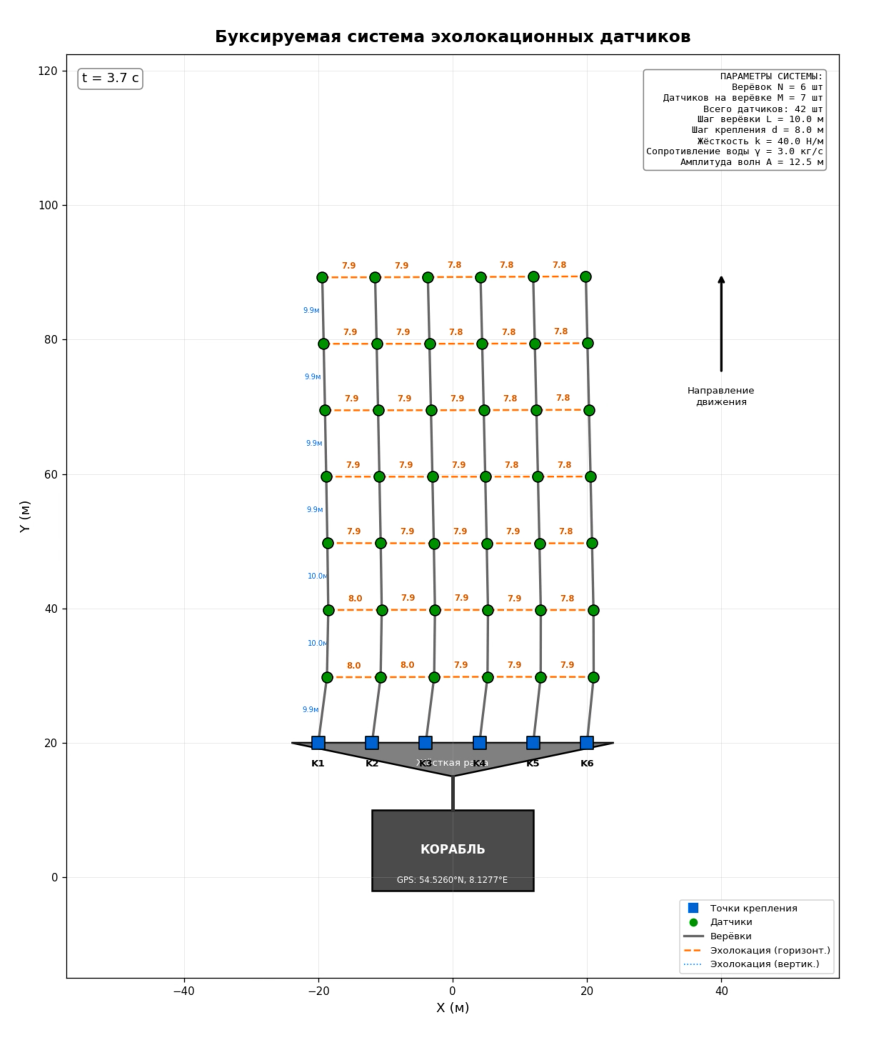
\includegraphics[width=\textwidth]{simulation_screenshot.png}
        \end{column}
\end{frame}

% ===========================================================================
% РАЗДЕЛ 3: АЛГОРИТМ ТРИАНГУЛЯЦИИ
% ===========================================================================
\section{Алгоритм триангуляции}

\begin{frame}{Постановка задачи триангуляции}
    \textbf{Дано:}
    \begin{itemize}
        \item Позиции точек крепления $\mathbf{R}_i$ (из GPS)
        \item Вертикальные расстояния $d_{i,j}^{(v)} = |\mathbf{r}_{i,j} - \mathbf{r}_{i,j-1}|$
        \item Горизонтальные расстояния $d_{i,j}^{(h)} = |\mathbf{r}_{i+1,j} - \mathbf{r}_{i,j}|$
    \end{itemize}
    
    \vspace{0.5cm}
    \textbf{Найти:}
    \begin{itemize}
        \item Координаты всех датчиков $\mathbf{r}_{i,j} = (x_{i,j}, y_{i,j})$
    \end{itemize}
    
    \vspace{0.5cm}
    \textbf{Подход:} Последовательная триангуляция --- восстанавливаем координаты строка за строкой, используя уже известные позиции.
\end{frame}

\begin{frame}{Триангуляция по двум точкам}
    \textbf{Задача:} Найти точку $\mathbf{r}$, зная расстояния до двух известных точек $\mathbf{p}_1$ и $\mathbf{p}_2$.
    
    \vspace{0.3cm}
    \textbf{Система уравнений:}
    \[
    \begin{cases}
        |\mathbf{r} - \mathbf{p}_1| = d_1 \\
        |\mathbf{r} - \mathbf{p}_2| = d_2
    \end{cases}
    \]
    
    \vspace{0.3cm}
    \textbf{Решение} (в локальной системе координат):
    \[
    x = \frac{d_1^2 - d_2^2 + D^2}{2D}, \quad y = \pm\sqrt{d_1^2 - x^2}
    \]
    где $D = |\mathbf{p}_2 - \mathbf{p}_1|$
    
    \vspace{0.3cm}
    \textbf{Выбор знака:} Используем априорную информацию о геометрии системы.
\end{frame}

\begin{frame}{Математическая модель: система уравнений}
    \textbf{Для каждого датчика $(i, j)$ имеем уравнения связи:}
    
    \vspace{0.3cm}
    Вертикальная связь (с верхним соседом):
    \[
    (x_{i,j} - x_{i,j-1})^2 + (y_{i,j} - y_{i,j-1})^2 = (d_{i,j}^{(v)})^2
    \]
    
    Горизонтальная связь (с левым соседом):
    \[
    (x_{i,j} - x_{i-1,j})^2 + (y_{i,j} - y_{i-1,j})^2 = (d_{i-1,j}^{(h)})^2
    \]
    
    Диагональная связь:
    \[
    (x_{i,j} - x_{i-1,j-1})^2 + (y_{i,j} - y_{i-1,j-1})^2 = (d_{i-1,j-1}^{(d)})^2
    \]
    
    \vspace{0.3cm}
    \textbf{Всего:} $2 \times N \times M$ неизвестных, связанных нелинейными уравнениями.
\end{frame}

\begin{frame}{Геометрическая интерпретация}
    \begin{columns}
        \begin{column}{0.5\textwidth}
            \textbf{Задача:} найти точку $\mathbf{r}$, зная расстояния $d_1$ и $d_2$ до известных точек.
            
            \vspace{0.2cm}
            \textbf{Геометрически:}
            \begin{itemize}
                \item Точки на расстоянии $d_1$ от $\mathbf{p}_1$ образуют окружность
                \item Точки на расстоянии $d_2$ от $\mathbf{p}_2$ образуют окружность
                \item Решение --- пересечение окружностей
            \end{itemize}
            
            \vspace{0.2cm}
            Две окружности дают два решения --- выбираем по геометрии системы.
        \end{column}
        \begin{column}{0.5\textwidth}
            \centering
            \begin{tikzpicture}[scale=0.8]
                % Точки p1 и p2
                \fill[blue] (0, 0) circle (0.1) node[below left] {$\mathbf{p}_1$};
                \fill[blue] (4, 0) circle (0.1) node[below right] {$\mathbf{p}_2$};
                
                % Окружности
                \draw[orange, thick] (0, 0) circle (2.5);
                \draw[cyan, thick] (4, 0) circle (2);
                
                % Точки пересечения
                \fill[red] (2.05, 1.95) circle (0.12) node[above right] {$\mathbf{r}$};
                \fill[gray] (2.05, -1.95) circle (0.08);
                
                % Радиусы
                \draw[orange, dashed] (0, 0) -- (2.05, 1.95) node[midway, left] {$d_1$};
                \draw[cyan, dashed] (4, 0) -- (2.05, 1.95) node[midway, right] {$d_2$};
                
                % Расстояние D
                \draw[<->] (0, -0.5) -- (4, -0.5) node[midway, below] {$D$};
            \end{tikzpicture}
        \end{column}
    \end{columns}
\end{frame}

\begin{frame}{Вывод формулы триангуляции}
    \textbf{Дано:} $\mathbf{p}_1 = (0, 0)$, $\mathbf{p}_2 = (D, 0)$, расстояния $d_1$, $d_2$.
    
    \vspace{0.3cm}
    \textbf{Система уравнений:}
    \[
    \begin{cases}
        x^2 + y^2 = d_1^2 \\
        (x - D)^2 + y^2 = d_2^2
    \end{cases}
    \]
    
    \[
    x^2 - (x - D)^2 = d_1^2 - d_2^2
    \]
    \[
    \boxed{x = \frac{d_1^2 - d_2^2 + D^2}{2D}}
    \]
    
    \textbf{Подставляем в первое уравнение:}
    \[
    \boxed{y = \pm\sqrt{d_1^2 - x^2}}
    \]
\end{frame}

\begin{frame}{Последовательный алгоритм решения}
    \textbf{Идея:} решаем систему последовательно, используя уже найденные координаты.
    
    \vspace{0.3cm}
    \textbf{Алгоритм:}
    \begin{enumerate}
        \item Начальные данные: координаты креплений $\mathbf{R}_1, \ldots, \mathbf{R}_N$ (из GPS)
        
        \item Для каждого ряда $j = 1, 2, \ldots, M$:
        \begin{itemize}
            \item Для $i = 1$: используем только вертикальное расстояние
            \[
            \mathbf{r}_{1,j} = \mathbf{r}_{1,j-1} + d_{1,j}^{(v)} \cdot \mathbf{e}_{\text{вниз}}
            \]
            \item Для $i = 2, \ldots, N$: триангуляция по двум точкам
            \[
            \mathbf{r}_{i,j} = \text{Triangulate}(\mathbf{r}_{i,j-1}, d_{i,j}^{(v)}, \mathbf{r}_{i-1,j}, d_{i-1,j}^{(h)})
            \]
        \end{itemize}
    \end{enumerate}
    
    \vspace{0.3cm}
    \textbf{Сложность:} $O(N \times M)$ --- линейная по числу датчиков.
\end{frame}

\begin{frame}{Результат триангуляции}
    \begin{columns}
        \begin{column}{0.5\textwidth}
            \textbf{Сравнение позиций:}
            \begin{itemize}
                \item Зелёные точки --- истинные позиции
                \item Красные крестики --- восстановленные
                \item Линии --- ошибки позиционирования
            \end{itemize}
            
            \vspace{0.5cm}
            \textbf{Метрики:}
            \begin{itemize}
                \item RMSE: 0.42 м
                \item Максимальная ошибка: 0.81 м
            \end{itemize}
        \end{column}
        \begin{column}{0.5\textwidth}
            \centering
            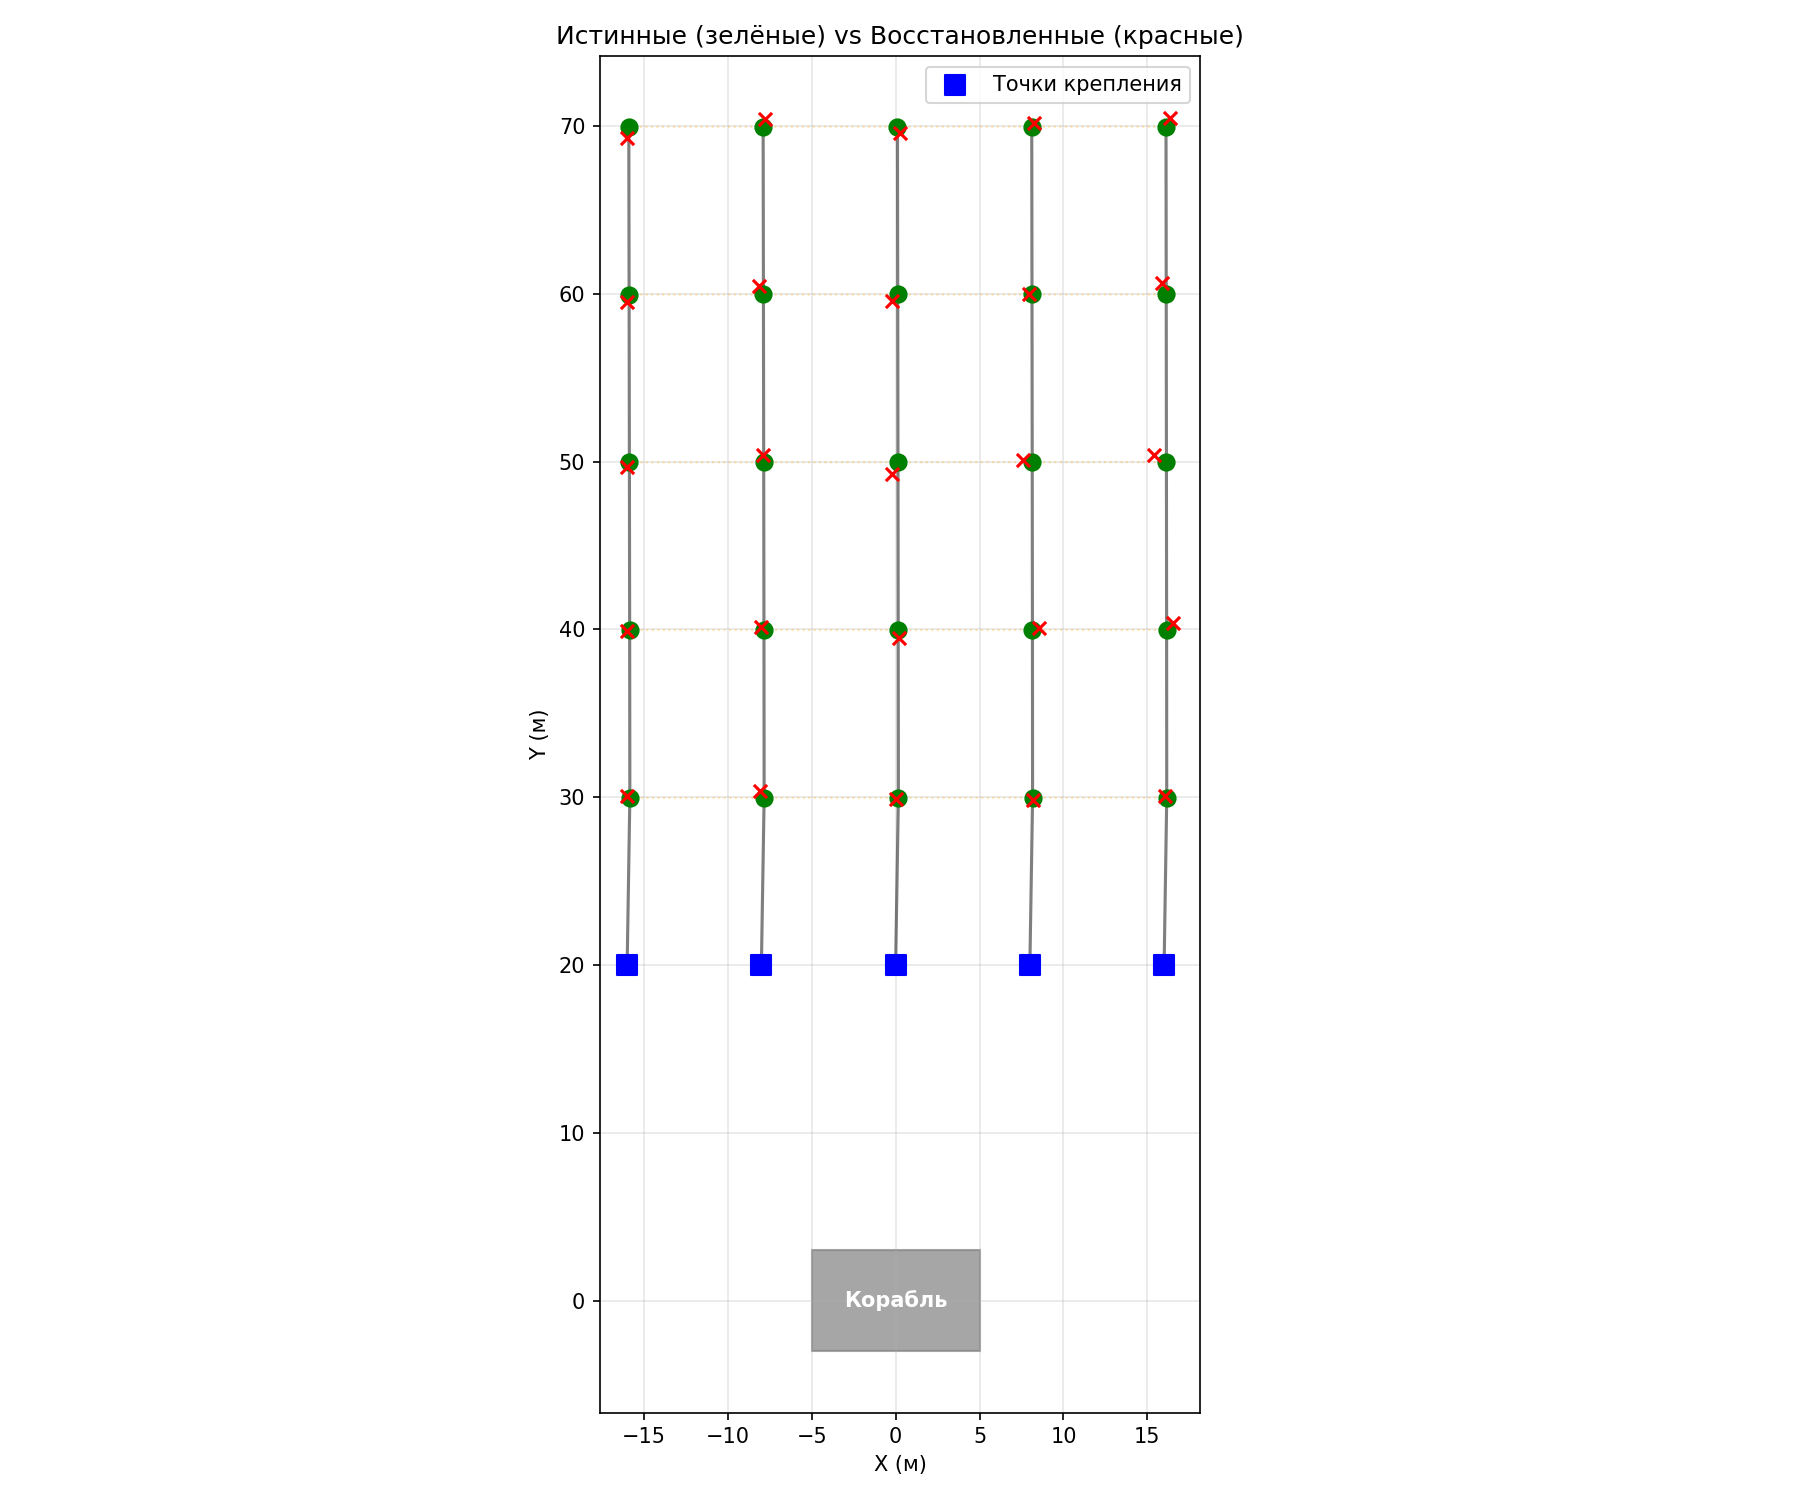
\includegraphics[width=\textwidth]{state_comparison.png}
        \end{column}
    \end{columns}
\end{frame}

% ===========================================================================
% РАЗДЕЛ 4: ФИЛЬТР КАЛМАНА
% ===========================================================================
\section{Фильтр Калмана}

\begin{frame}{Фильтр Калмана}
    \textbf{Проблема триангуляции:}
    \begin{itemize}
        \item Каждый момент времени обрабатывается независимо
        \item Шум измерений напрямую влияет на результат
        \item Не используется информация о движении датчиков
    \end{itemize}
    
    \vspace{0.5cm}
    \textbf{фильтр Калмана:}
    \begin{itemize}
        \item Сглаживает шум измерений
        \item Предсказывает положение на основе модели движения
        \item Оценивает скорость датчиков
        \item Даёт оценку неопределённости (доверительные интервалы)
    \end{itemize}
\end{frame}

\begin{frame}{Математическая модель фильтра Калмана}
    \textbf{Вектор состояния} --- положение и скорость датчика:
    \[
    \mathbf{x} = \begin{bmatrix} x \\ y \\ v_x \\ v_y \end{bmatrix}
    \]
    
    \vspace{0.3cm}
    \textbf{Модель динамики} (постоянная скорость):
    \[
    \mathbf{x}_{k+1} = \mathbf{F} \mathbf{x}_k + \mathbf{w}_k
    \]
    
    где $\mathbf{w}_k \sim \mathcal{N}(0, \mathbf{Q})$ --- случайные ускорения (шум процесса).
    
    \vspace{0.3cm}
    \textbf{Смысл:} за время $\Delta t$ координата изменяется на $v \cdot \Delta t$, скорость почти постоянна.
\end{frame}

\begin{frame}{Матрица перехода состояния}
    \textbf{Уравнения движения:}
    \[
    \begin{cases}
        x_{k+1} = x_k + v_x \cdot \Delta t \\
        y_{k+1} = y_k + v_y \cdot \Delta t \\
        v_{x,k+1} = v_{x,k} \\
        v_{y,k+1} = v_{y,k}
    \end{cases}
    \]
    
    \vspace{0.3cm}
    \textbf{В матричной форме:}
    \[
    \begin{bmatrix} x \\ y \\ v_x \\ v_y \end{bmatrix}_{k+1} = 
    \underbrace{\begin{bmatrix} 
        1 & 0 & \Delta t & 0 \\ 
        0 & 1 & 0 & \Delta t \\ 
        0 & 0 & 1 & 0 \\ 
        0 & 0 & 0 & 1 
    \end{bmatrix}}_{\mathbf{F}}
    \begin{bmatrix} x \\ y \\ v_x \\ v_y \end{bmatrix}_{k}
    \]
\end{frame}

\begin{frame}{Модель измерений}
    \textbf{Измерение} --- расстояние до известной точки:
    \[
    z_k = h(\mathbf{x}_k) + v_k
    \]
    
    где функция измерения:
    \[
    h(\mathbf{x}) = \sqrt{(x - x_a)^2 + (y - y_a)^2}
    \]
    
    и $v_k \sim \mathcal{N}(0, R)$ --- шум измерений.
    
    \vspace{0.5cm}
    \textbf{}В связи с нелинейностью функции $h(\mathbf{x})$ необходимо использовать \textbf{расширенный фильтр Калмана} (EKF) с линеаризацией. \textbf
    
\end{frame}

\begin{frame}{Линеаризация: якобиан измерения}
    \textbf{Якобиан} --- матрица частных производных:
    \[
    \mathbf{H} = \frac{\partial h}{\partial \mathbf{x}} = \begin{bmatrix} 
        \dfrac{\partial h}{\partial x} & 
        \dfrac{\partial h}{\partial y} & 
        \dfrac{\partial h}{\partial v_x} & 
        \dfrac{\partial h}{\partial v_y} 
    \end{bmatrix}
    \]
    
    \vspace{0.3cm}
    \textbf{Вычисляем производные:}
    \[
    \frac{\partial h}{\partial x} = \frac{x - x_a}{\sqrt{(x-x_a)^2 + (y-y_a)^2}} = \frac{x - x_a}{d}
    \]
    
    \vspace{0.3cm}
    \textbf{Результат:}
    \[
    \mathbf{H} = \begin{bmatrix} \dfrac{x - x_a}{d} & \dfrac{y - y_a}{d} & 0 & 0 \end{bmatrix}
    \]
    
    Скорость не влияет на текущее измерение расстояния.
\end{frame}

\begin{frame}{Алгоритм EKF: предсказание}
    \textbf{Шаг 1: Предсказание состояния}
    \[
    \hat{\mathbf{x}}_{k|k-1} = \mathbf{F} \hat{\mathbf{x}}_{k-1|k-1}
    \]
    
    Предсказываем новое положение на основе предыдущего и модели движения.
    
    \vspace{0.5cm}
    \textbf{Шаг 2: Предсказание ковариации}
    \[
    \mathbf{P}_{k|k-1} = \mathbf{F} \mathbf{P}_{k-1|k-1} \mathbf{F}^T + \mathbf{Q}
    \]
    
    Неопределённость растёт из-за шума процесса $\mathbf{Q}$.
    
    \vspace{0.5cm}
    \textit{Индекс $k|k-1$ означает: оценка на шаг $k$ по данным до шага $k-1$.}
\end{frame}

\begin{frame}{Алгоритм EKF: коррекция}
    \textbf{Шаг 3: Коэффициент Калмана}
    \[
    \mathbf{K}_k = \mathbf{P}_{k|k-1} \mathbf{H}_k^T (\mathbf{H}_k \mathbf{P}_{k|k-1} \mathbf{H}_k^T + R)^{-1}
    \]
    
    Определяет, насколько доверять измерению или предсказанию.
    
    \vspace{0.1cm}
    \textbf{Шаг 4: Обновление состояния}
    \[
    \hat{\mathbf{x}}_{k|k} = \hat{\mathbf{x}}_{k|k-1} + \mathbf{K}_k \underbrace{(z_k - h(\hat{\mathbf{x}}_{k|k-1}))}_{\text{невязка}}
    \]
    
    Корректируем предсказание на основе разницы между измерением и ожиданием.
    
    \vspace{0.1cm}
    \textbf{Шаг 5: Обновление ковариации}
    \[
    \mathbf{P}_{k|k} = (\mathbf{I} - \mathbf{K}_k \mathbf{H}_k) \mathbf{P}_{k|k-1}
    \]
    
    Неопределённость уменьшается после получения измерения.
\end{frame}

\begin{frame}{Матрица шума процесса $\mathbf{Q}$}
    \textbf{Модель:} случайные ускорения с дисперсией $\sigma_a^2$.
    
    \textbf{Вывод:} интегрируем ускорение дважды для получения влияния на координаты.
    
    \begin{equation*}
        \scalebox{0.8}{$
        \mathbf{Q} = \sigma_a^2 \begin{bmatrix} 
            \dfrac{\Delta t^4}{4} & 0 & \dfrac{\Delta t^3}{2} & 0 \\[0.3cm]
            0 & \dfrac{\Delta t^4}{4} & 0 & \dfrac{\Delta t^3}{2} \\[0.3cm]
            \dfrac{\Delta t^3}{2} & 0 & \Delta t^2 & 0 \\[0.3cm]
            0 & \dfrac{\Delta t^3}{2} & 0 & \Delta t^2
        \end{bmatrix}
        $}
    \end{equation*}
    
    \textbf{Диагональные элементы:} дисперсии координат и скоростей.
    
    \textbf{Недиагональные элементы:} корреляция между координатой и скоростью.
\end{frame}

\begin{frame}{Использование фильтра Калмана}
    \begin{columns}
        \begin{column}{0.5\textwidth}
            \textbf{Если $R$ большое} (шумные измерения):
            \begin{itemize}
                \item $\mathbf{K}$ маленький
                \item Больше доверяем предсказанию
                \item Сильное сглаживание
            \end{itemize}
            
            \vspace{0.5cm}
            \textbf{Если $R$ маленькое} (точные измерения):
            \begin{itemize}
                \item $\mathbf{K}$ большой
                \item Больше доверяем измерению
                \item Слабое сглаживание
            \end{itemize}
        \end{column}
        \begin{column}{0.5\textwidth}
            \textbf{Если $\mathbf{Q}$ большое} (непредсказуемое движение):
            \begin{itemize}
                \item Предсказание ненадёжно
                \item Больше доверяем измерениям
            \end{itemize}
            
            \vspace{0.5cm}
            \textbf{Если $\mathbf{Q}$ маленькое} (плавное движение):
            \begin{itemize}
                \item Предсказание надёжно
                \item Сильное сглаживание траектории
            \end{itemize}
        \end{column}
    \end{columns}
\end{frame}

\begin{frame}{Расширенный фильтр Калмана (EKF)}
    \textbf{Состояние датчика:} $\mathbf{x} = [x, y, v_x, v_y]^T$
    
    \vspace{0.3cm}
    \textbf{Модель движения} (постоянная скорость):
    \[
    \mathbf{x}_{k+1} = \mathbf{F} \mathbf{x}_k + \mathbf{w}_k, \quad \mathbf{F} = \begin{bmatrix} 1 & 0 & \Delta t & 0 \\ 0 & 1 & 0 & \Delta t \\ 0 & 0 & 1 & 0 \\ 0 & 0 & 0 & 1 \end{bmatrix}
    \]
    
    \vspace{0.3cm}
    \textbf{Модель измерений} (нелинейная):
    \[
    z_k = h(\mathbf{x}_k) + v_k, \quad h(\mathbf{x}) = \|\mathbf{r} - \mathbf{r}_{\text{anchor}}\|
    \]

    \begin{itemize}
        \item $\mathbf{w}_k \sim \mathcal{N}(0, \mathbf{Q})$ --- шум процесса
        \item $v_k \sim \mathcal{N}(0, R)$ --- шум измерений
    \end{itemize}
\end{frame}

\begin{frame}{Алгоритм EKF}
    \textbf{Шаг предсказания (Prediction):}
    \[
    \begin{aligned}
        \hat{\mathbf{x}}_{k|k-1} &= \mathbf{F} \hat{\mathbf{x}}_{k-1|k-1} \\
        \mathbf{P}_{k|k-1} &= \mathbf{F} \mathbf{P}_{k-1|k-1} \mathbf{F}^T + \mathbf{Q}
    \end{aligned}
    \]
    
    \vspace{0.3cm}
    \textbf{Шаг коррекции (Update):}
    \[
    \begin{aligned}
        \mathbf{K}_k &= \mathbf{P}_{k|k-1} \mathbf{H}_k^T (\mathbf{H}_k \mathbf{P}_{k|k-1} \mathbf{H}_k^T + R)^{-1} \\
        \hat{\mathbf{x}}_{k|k} &= \hat{\mathbf{x}}_{k|k-1} + \mathbf{K}_k (z_k - h(\hat{\mathbf{x}}_{k|k-1})) \\
        \mathbf{P}_{k|k} &= (\mathbf{I} - \mathbf{K}_k \mathbf{H}_k) \mathbf{P}_{k|k-1}
    \end{aligned}
    \]
    
    где $\mathbf{H}_k = \frac{\partial h}{\partial \mathbf{x}}$ --- Якобиан измерения
\end{frame}

\begin{frame}{Сравнение: Триангуляция vs Калман}
    \begin{columns}
        \begin{column}{0.5\textwidth}
            \textbf{Результаты:}
            \begin{table}
                \centering
                \begin{tabular}{lc}
                    \toprule
                    \textbf{Метод} & \textbf{RMSE} \\
                    \midrule
                    Триангуляция & 0.50 м \\
                    Фильтр Калмана & 0.28 м \\
                    \midrule
                    \textbf{Улучшение} & \textbf{43\%} \\
                    \bottomrule
                \end{tabular}
            \end{table}
            
            \vspace{0.3cm}
            \textbf{Преимущества Калмана:}
            \begin{itemize}
                \item Сглаживание шума
                \item Оценка скорости
                \item Оценка неопределённости
            \end{itemize}
        \end{column}
        \begin{column}{0.5\textwidth}
            \centering
            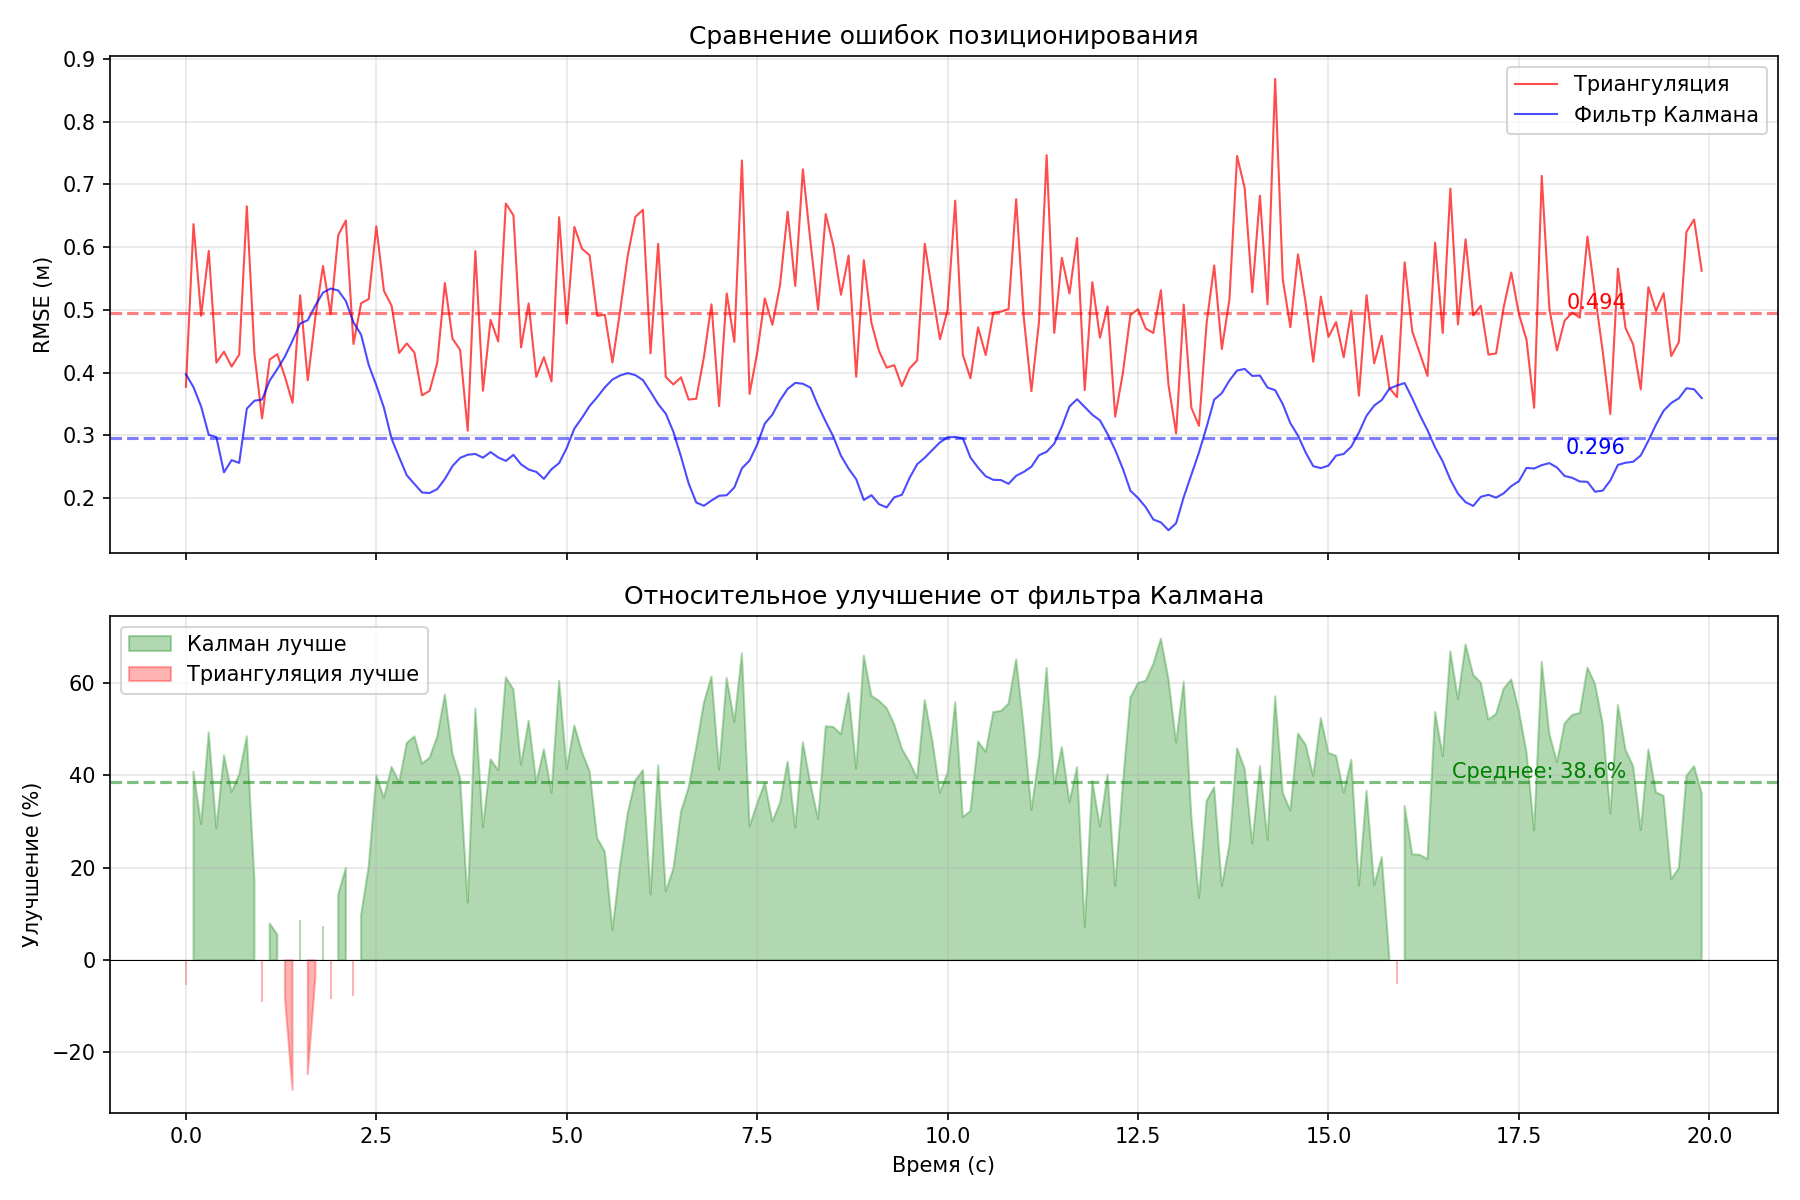
\includegraphics[width=\textwidth]{kalman_error_comparison.png}
        \end{column}
    \end{columns}
\end{frame}

\begin{frame}{Траектория датчика}
    \begin{columns}
        \begin{column}{0.45\textwidth}
            \textbf{Сравнение методов:}
            \begin{itemize}
                \item Зелёная линия --- истинная траектория
                \item Красные точки --- триангуляция (шум)
                \item Синяя линия --- фильтр Калмана (сглаживание)
            \end{itemize}
            
            \vspace{0.3cm}
            Калман эффективно фильтрует высокочастотный шум измерений.
        \end{column}
        \begin{column}{0.55\textwidth}
            \centering
            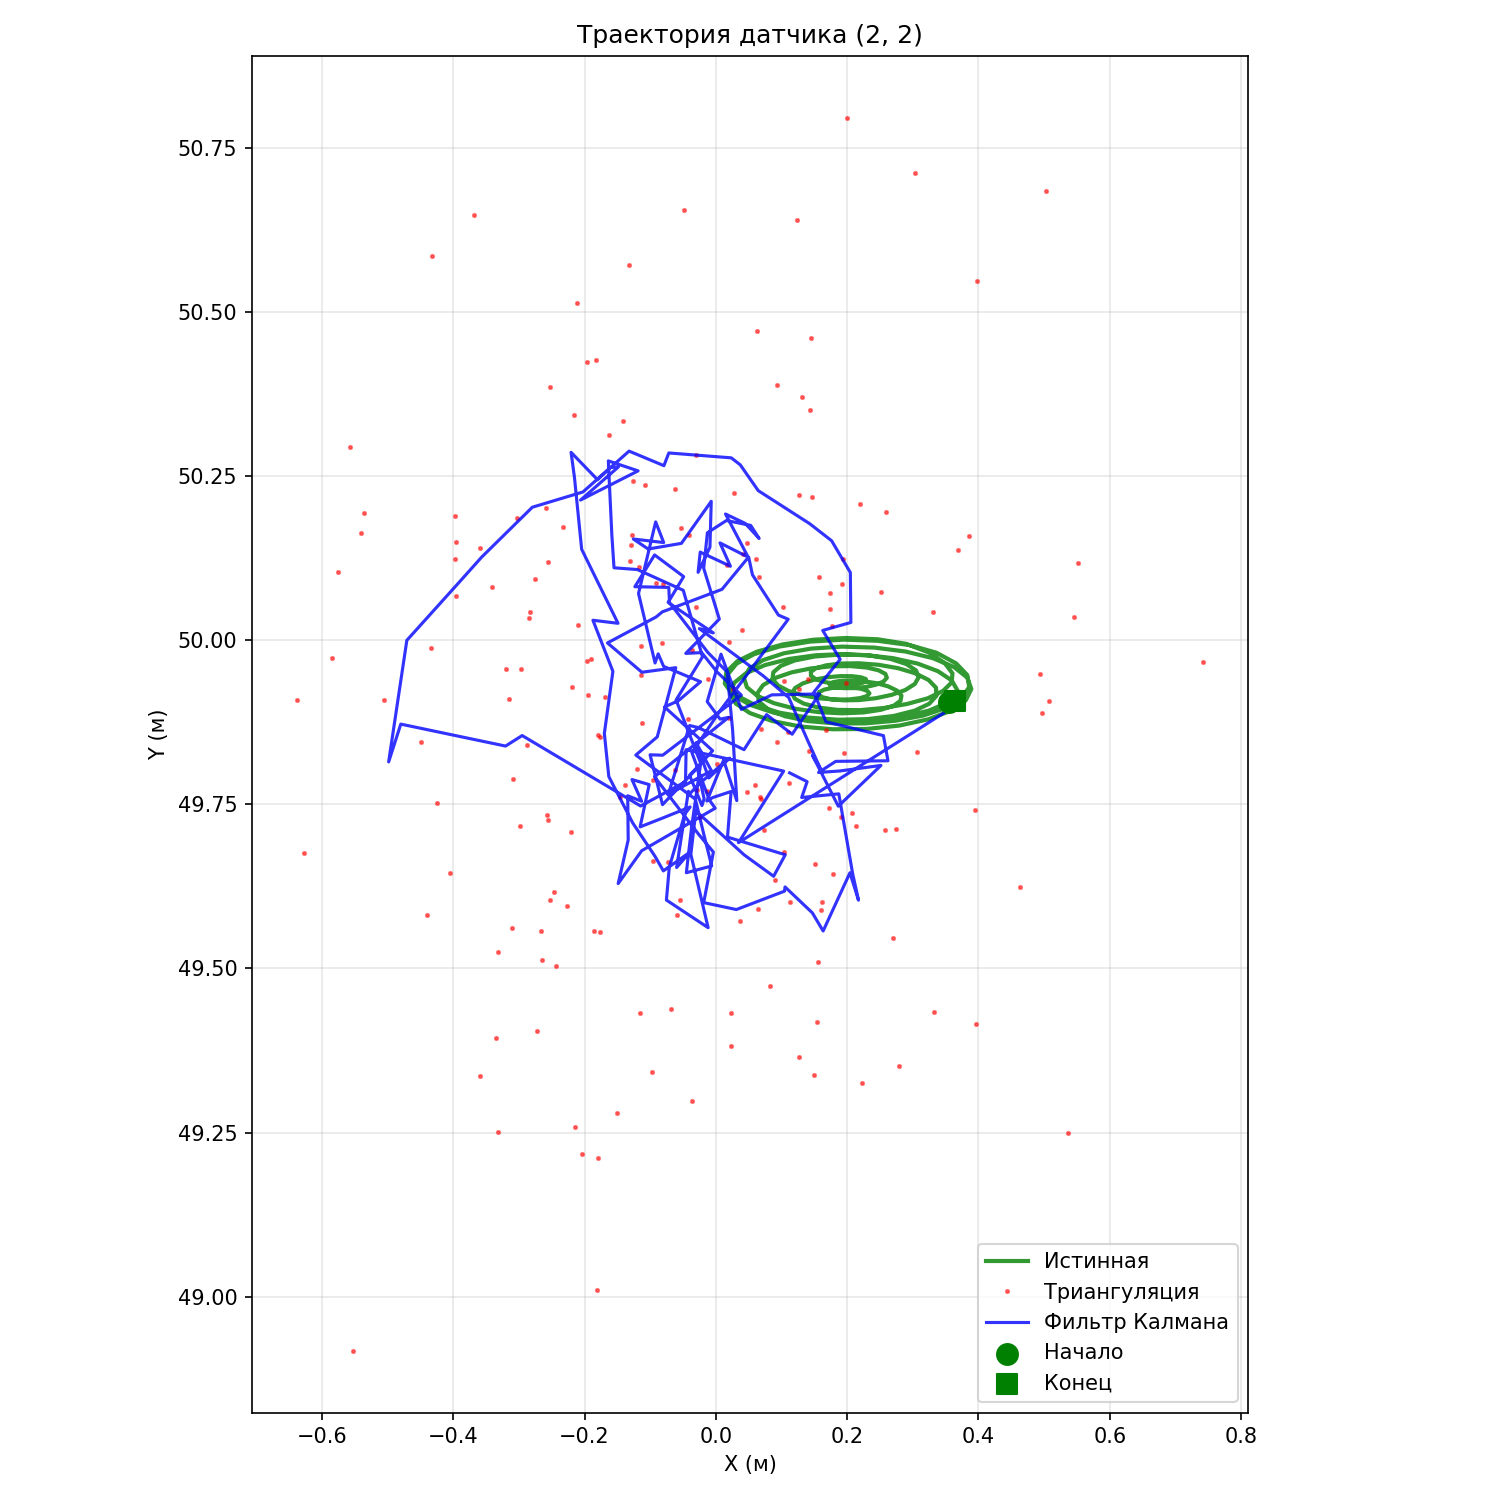
\includegraphics[width=\textwidth]{kalman_trajectory.png}
        \end{column}
    \end{columns}
\end{frame}

\begin{frame}{Эллипсы неопределённости}
    \centering
    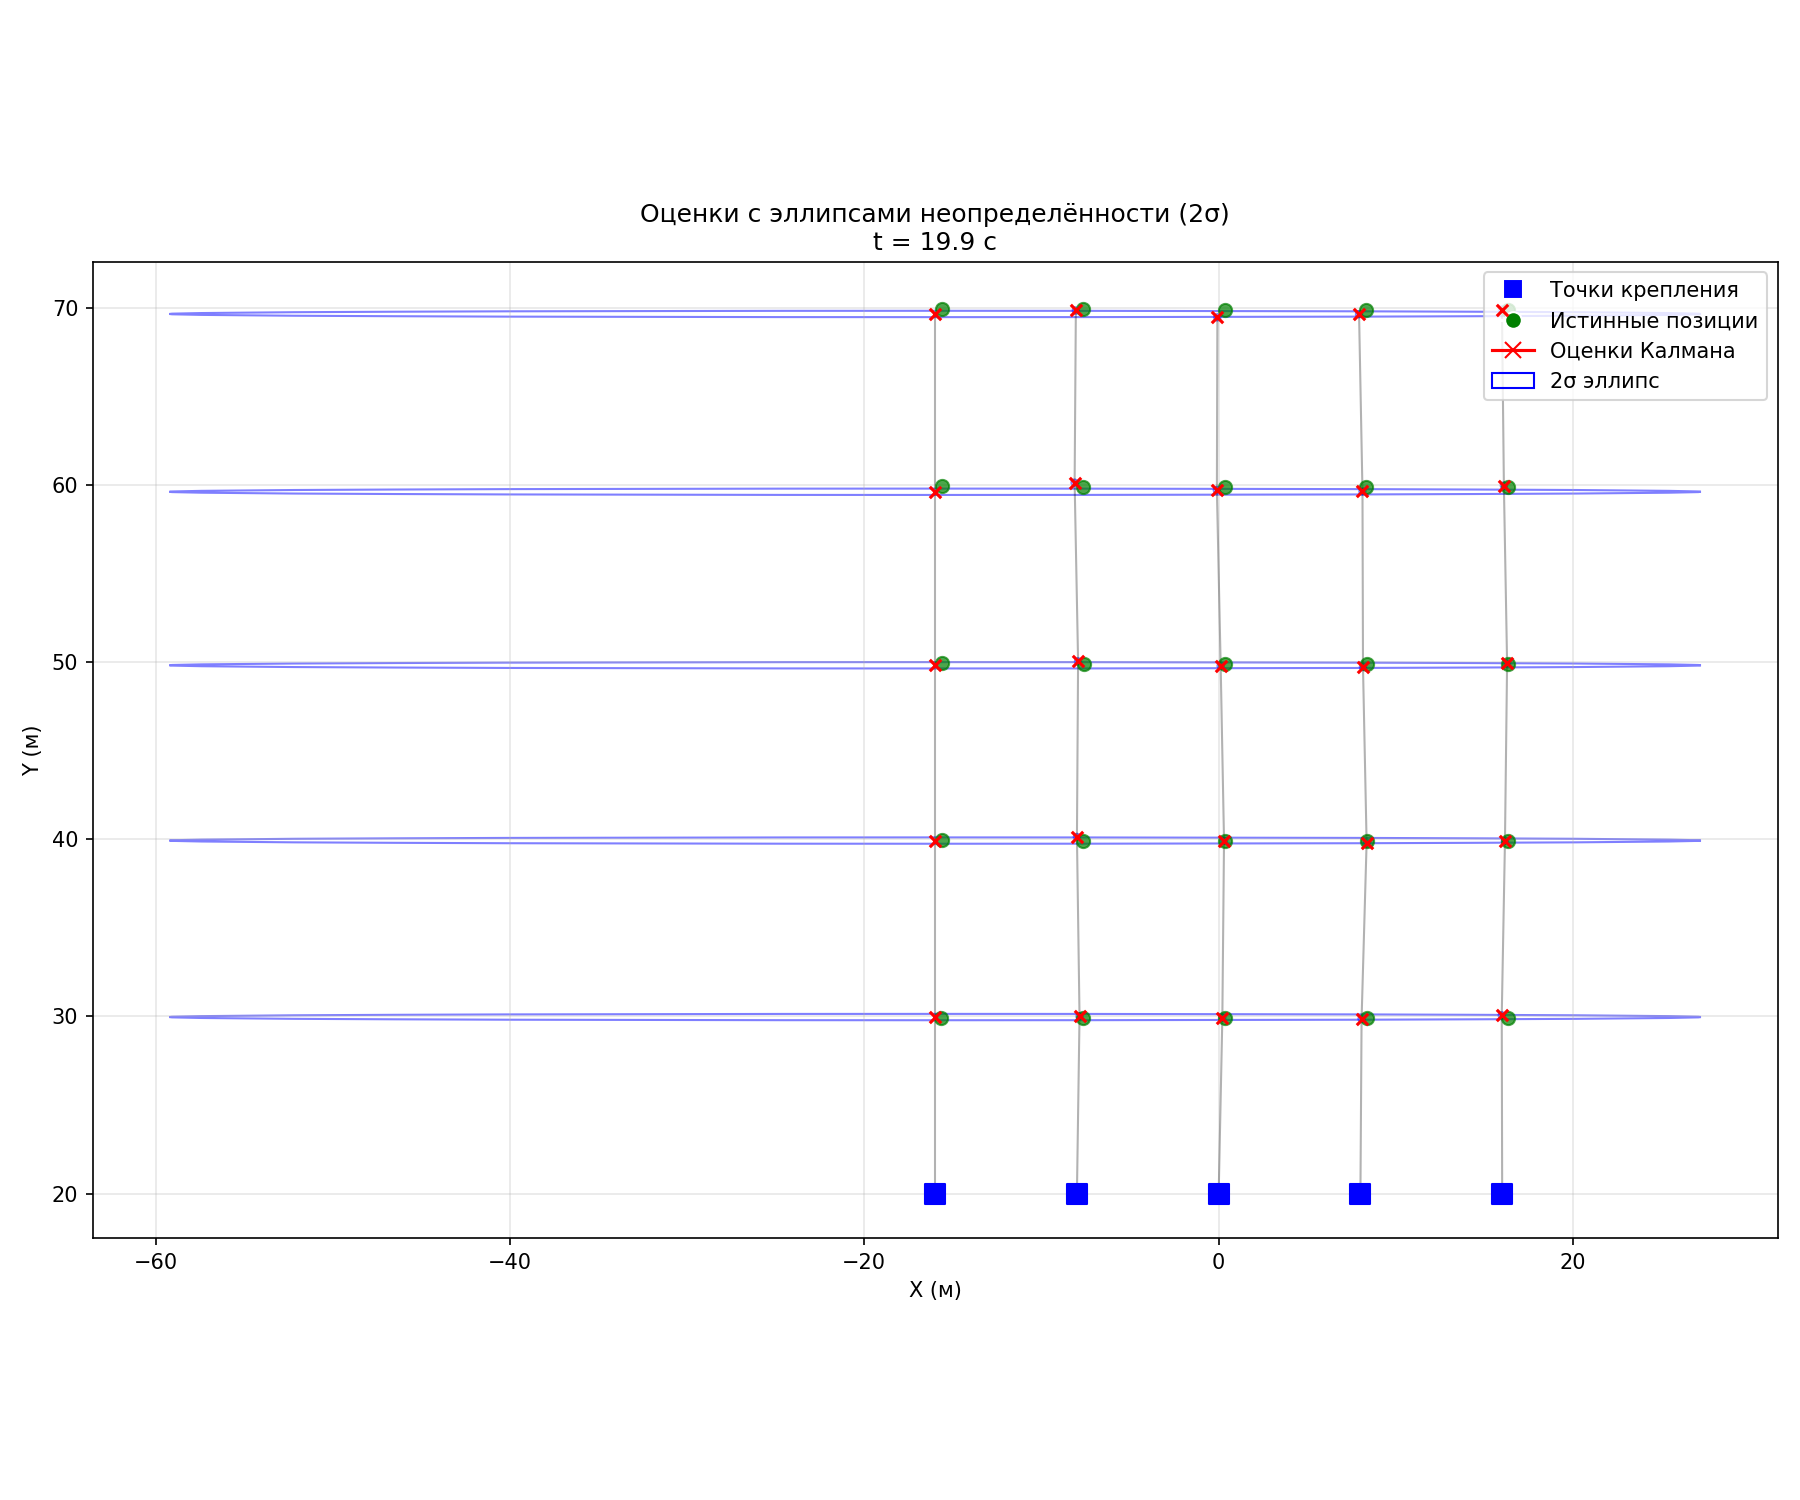
\includegraphics[width=0.7\textwidth]{kalman_uncertainty.png}
    
    \vspace{0.3cm}
    Эллипсы показывают 2$\sigma$ доверительные интервалы для каждого датчика.
\end{frame}

% ===========================================================================
% РАЗДЕЛ 5: АНАЛИЗ ПОГРЕШНОСТЕЙ
% ===========================================================================
\section{Анализ погрешностей}

\begin{frame}{Источники ошибок}
    \textbf{1. Базовый шум измерений:}
    \[
    \sigma_{\text{meas}} = 0.2 \text{ м}
    \]
    
    \vspace{0.3cm}
    \textbf{2. Накопление ошибок} (вдоль верёвки):
    \[
    \sigma_{\text{accum}}(j) = \sqrt{j} \cdot \sigma_{\text{meas}}
    \]
    
    \vspace{0.3cm}
    \textbf{3. Краевой эффект:}
    \[
    \text{Крайние верёвки } (i=1, i=N): \quad \sigma \times 1.3
    \]
    
    \vspace{0.3cm}
    \textbf{4. Геометрический фактор (PDOP):}
    \[
    \sigma_{\text{pos}} = \text{PDOP} \times \sigma_{\text{meas}}
    \]
\end{frame}

\begin{frame}{Распределение ошибок}
    \begin{columns}
        \begin{column}{0.45\textwidth}
            \textbf{Наблюдения:}
            \begin{itemize}
                \item Ошибки растут от креплений к свободным концам
                \item Крайние верёвки имеют большие ошибки
                \item Средний PDOP: 2.18
                \item Максимальный PDOP: 3.00
            \end{itemize}
            
            \vspace{0.3cm}
            \textbf{Уязвимые зоны:}
            \begin{itemize}
                \item Правый нижний угол
                \item Свободные концы
            \end{itemize}
        \end{column}
        \begin{column}{0.55\textwidth}
            \centering
            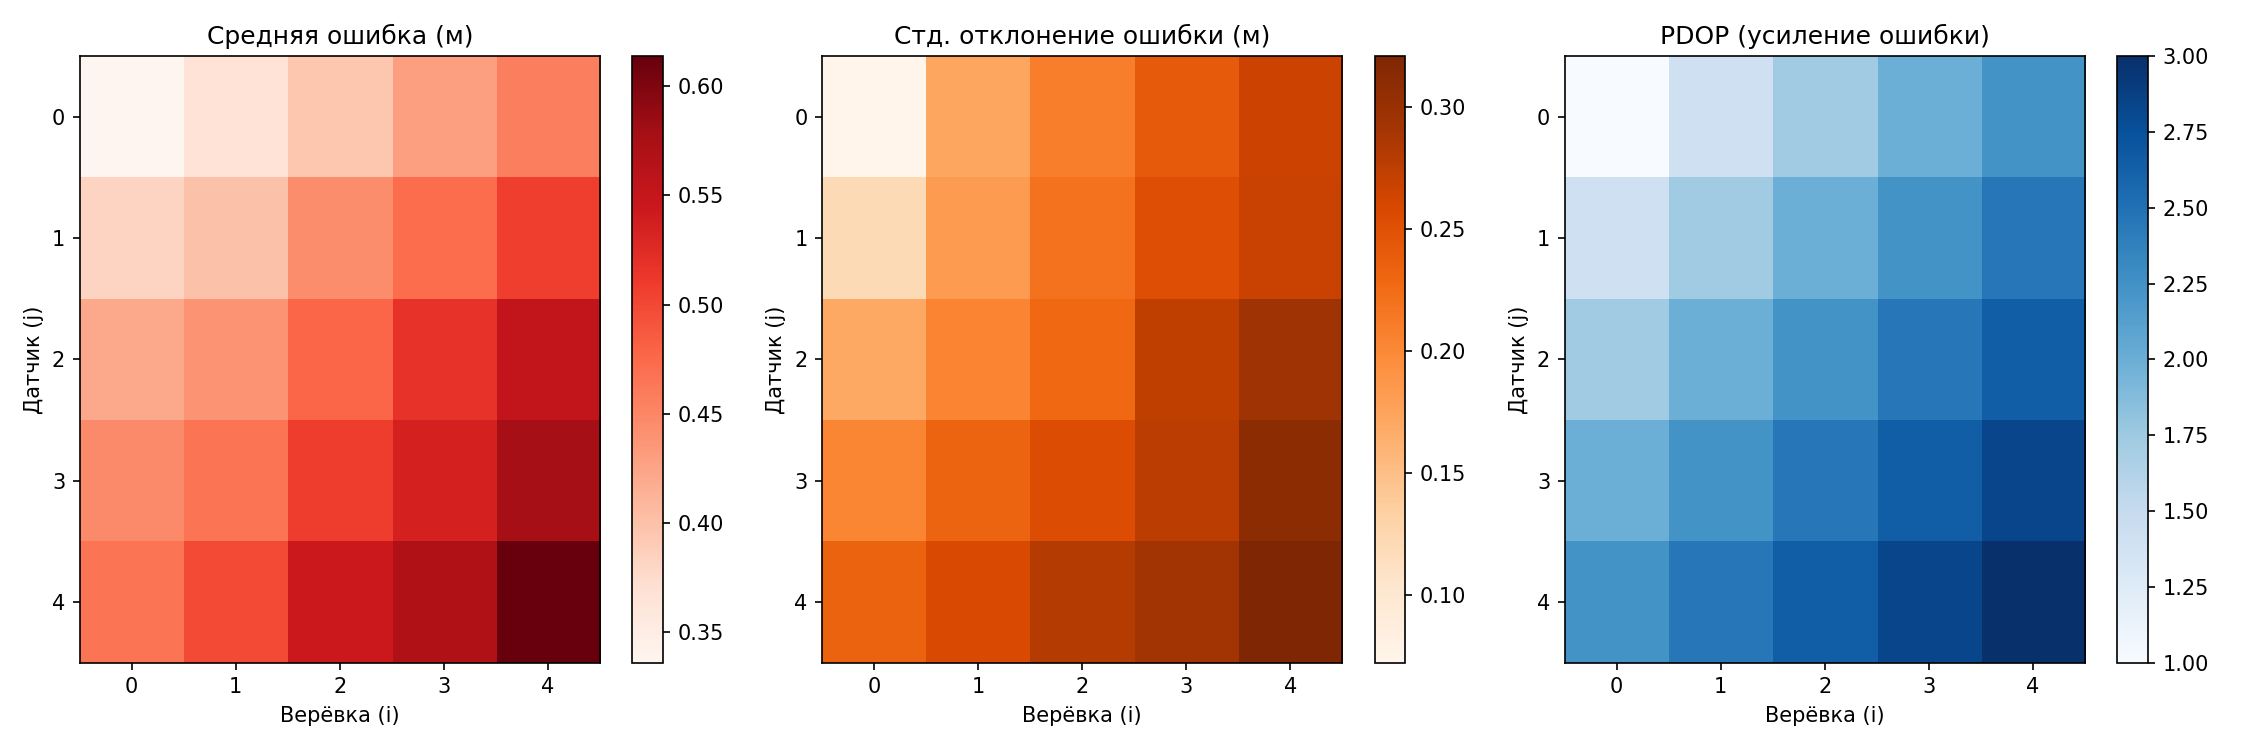
\includegraphics[width=\textwidth]{error_heatmap_detailed.png}
        \end{column}
    \end{columns}
\end{frame}

\begin{frame}{Факторы ошибок}
    \centering
    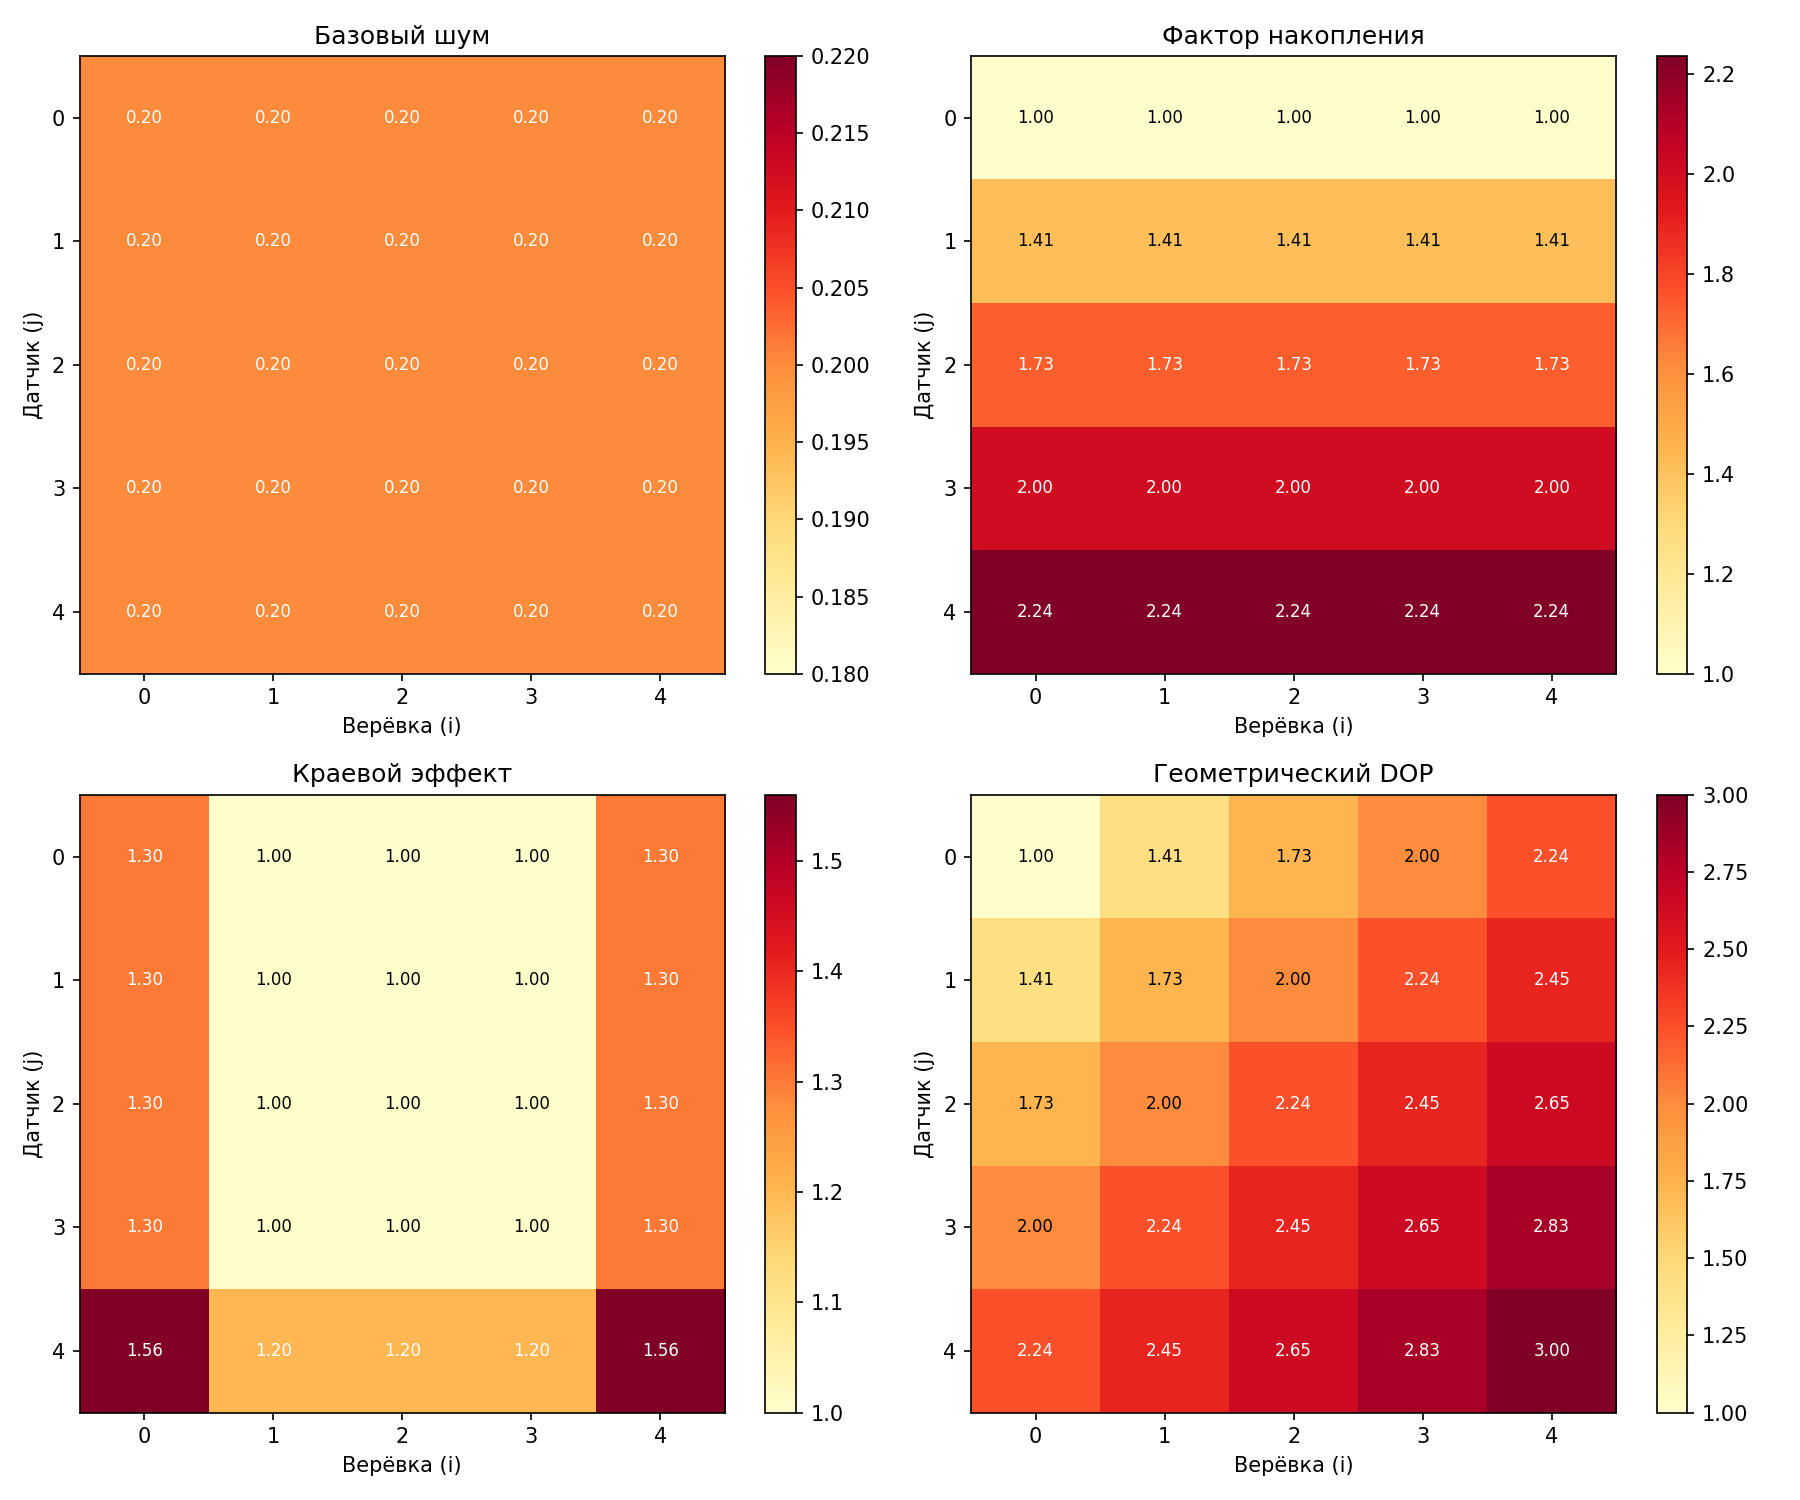
\includegraphics[width=0.85\textwidth]{error_sources.png}
    
    \vspace{0.2cm}
    Базовый шум, накопление, краевой эффект и геометрический DOP.
\end{frame}

\begin{frame}{Пространственное распределение ошибок}
    \centering
    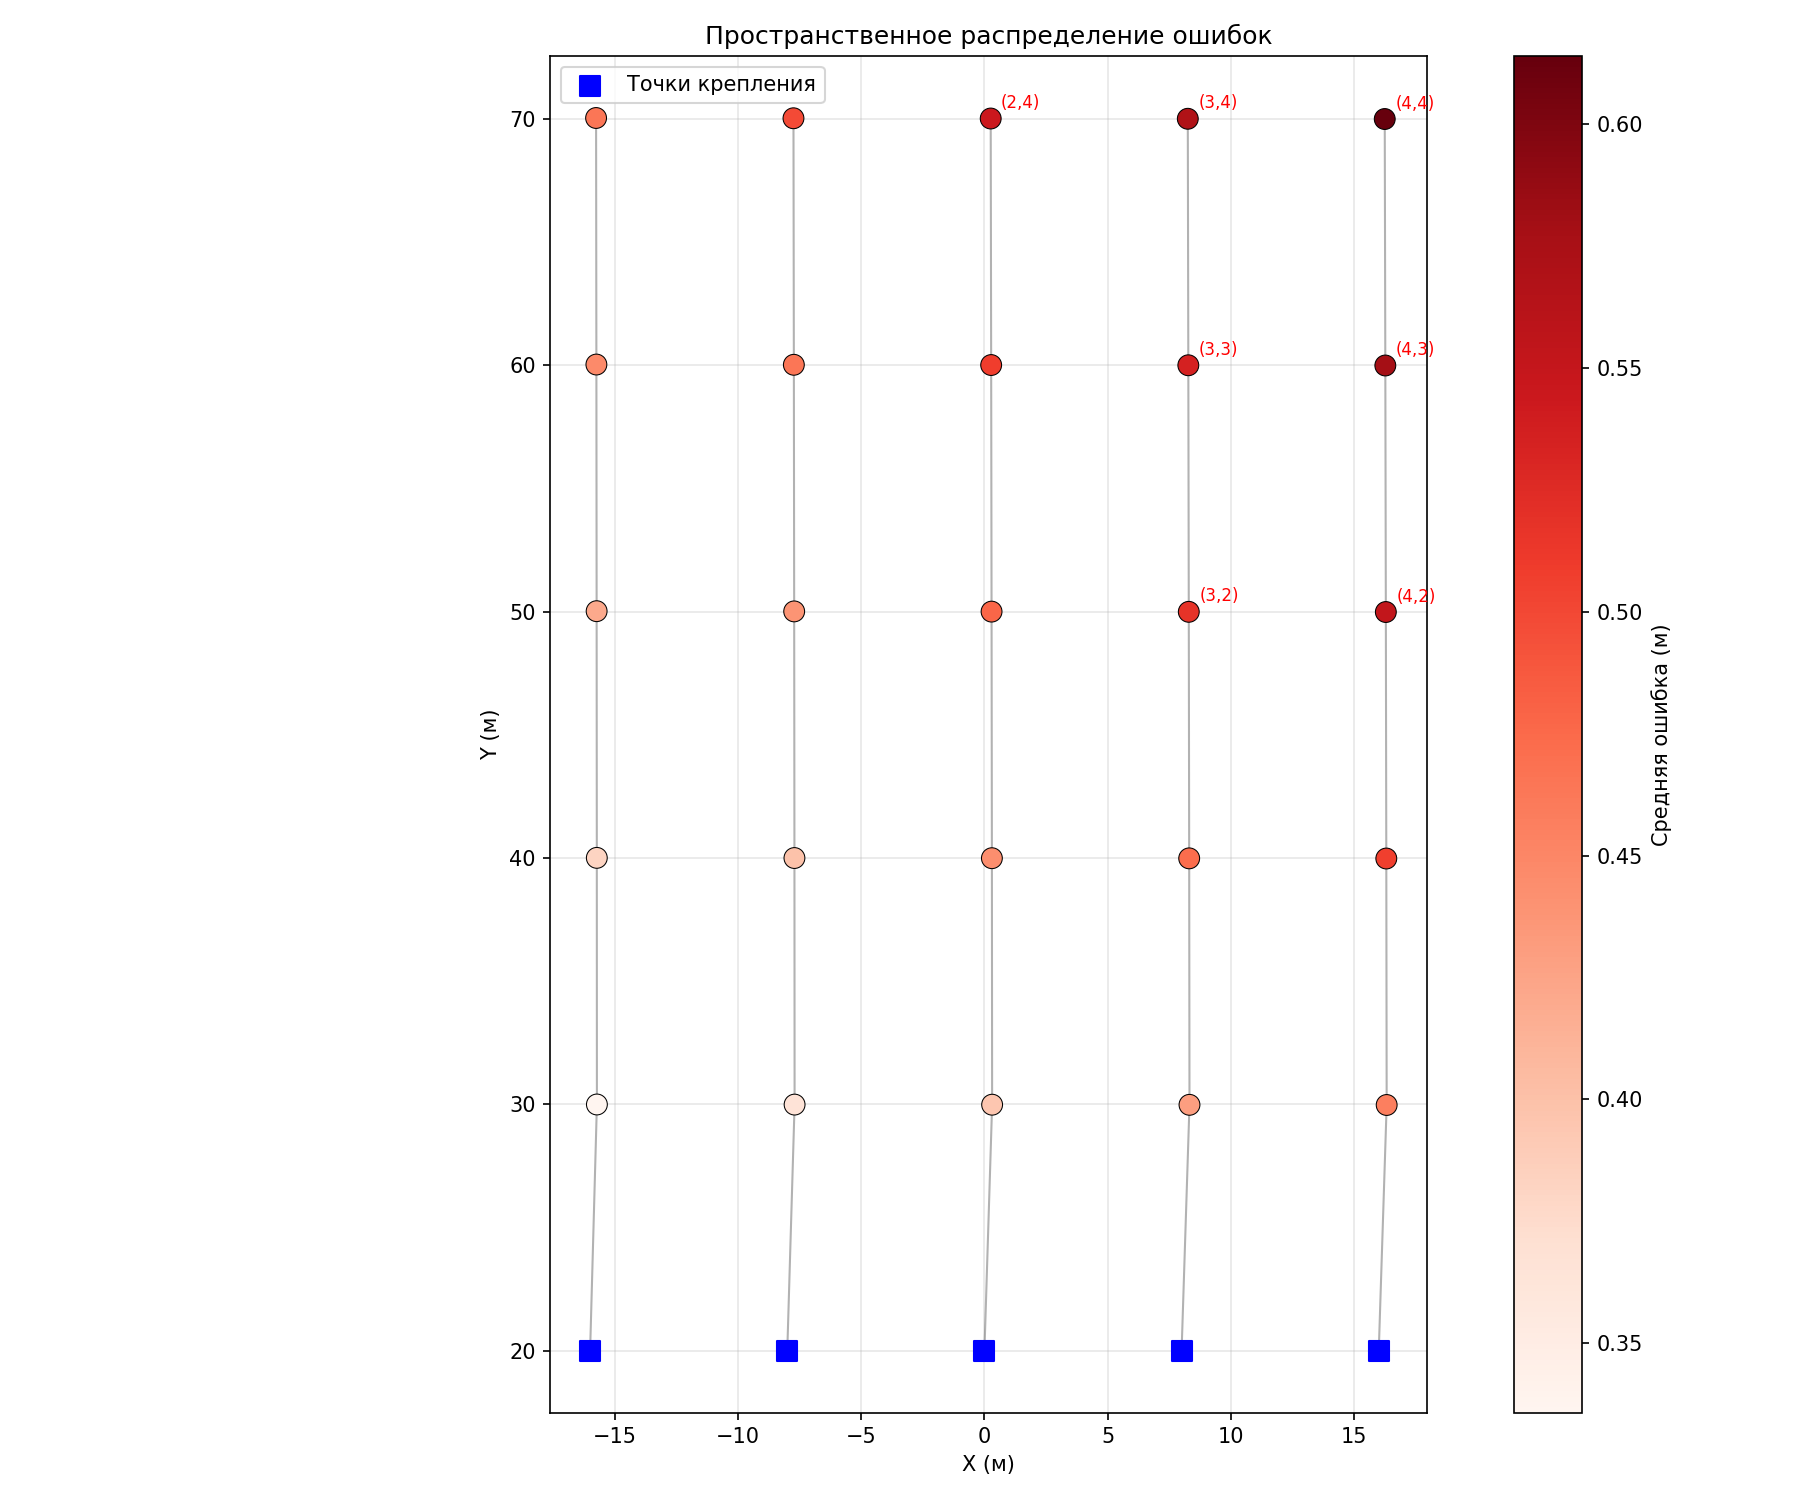
\includegraphics[width=0.7\textwidth]{spatial_errors.png}
    
    \vspace{0.3cm}
    Цвет точек показывает величину средней ошибки позиционирования.
\end{frame}

\begin{frame}{Чувствительность к шуму}
    \begin{columns}
        \begin{column}{0.45\textwidth}
            \textbf{Линейная зависимость:}
            \[
            \text{RMSE} \approx 2.93 \cdot \sigma
            \]
            
            \vspace{0.3cm}
            \textbf{Интерпретация:}
            \begin{itemize}
                \item Ошибка позиционирования примерно в 3 раза больше шума измерений
                \item Линейность подтверждает корректность модели
            \end{itemize}
        \end{column}
        \begin{column}{0.55\textwidth}
            \centering
            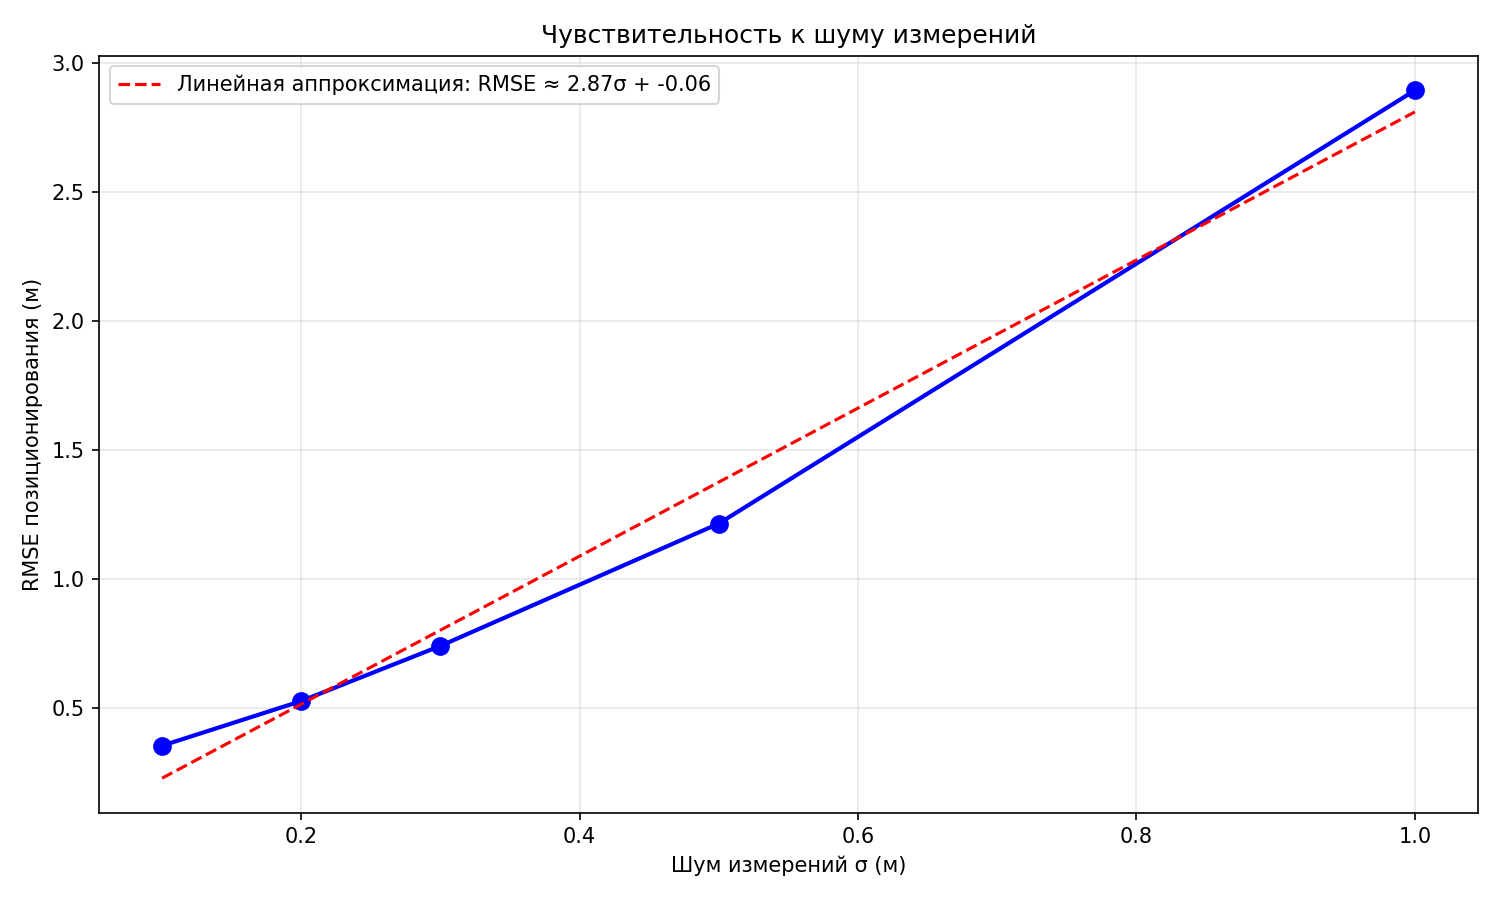
\includegraphics[width=\textwidth]{sensitivity_analysis.png}
        \end{column}
    \end{columns}
\end{frame}

\begin{frame}{Корреляция ошибок}
    \centering
    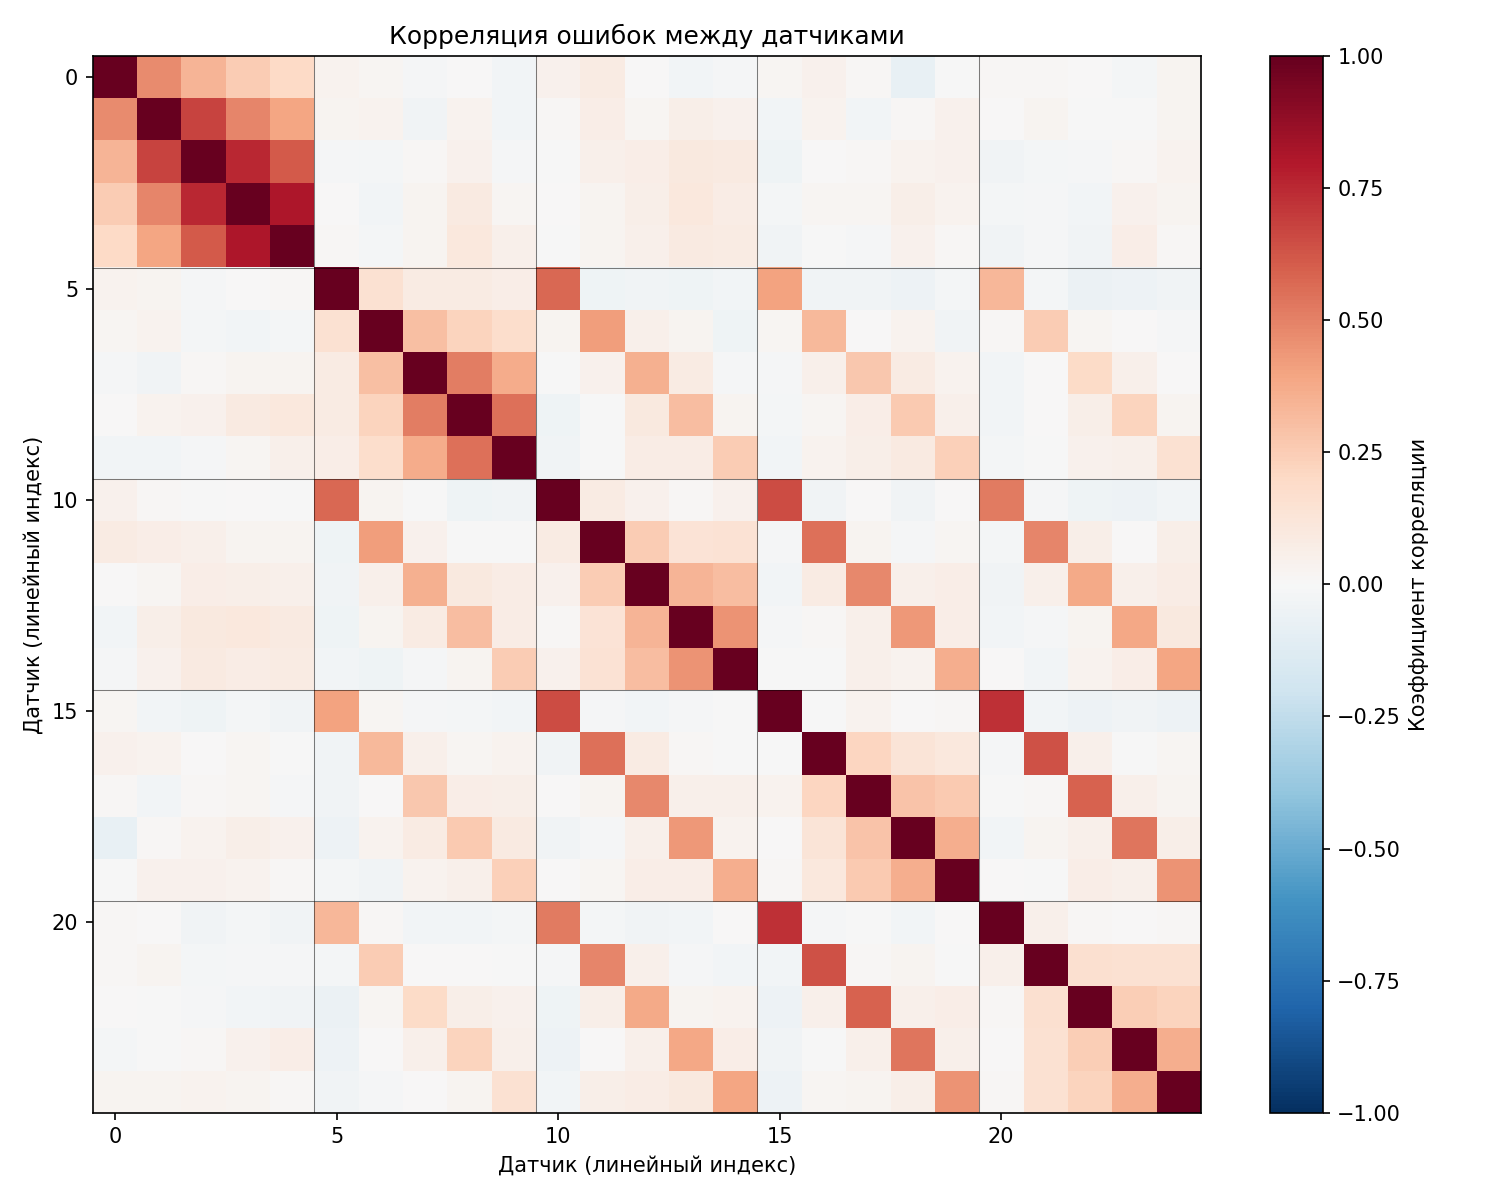
\includegraphics[width=0.55\textwidth]{error_correlation.png}
    
    \vspace{0.3cm}
    Сильная корреляция внутри верёвок, умеренная между соседними.
\end{frame}

% ===========================================================================
% РАЗДЕЛ 6: РЕЗУЛЬТАТЫ
% ===========================================================================
\section{Результаты}

\begin{frame}{Основные результаты}
    \textbf{1. Разработана физическая модель:}
    \begin{itemize}
        \item Система $4NM$ дифференциальных уравнений
        \item Учёт натяжения, сопротивления воды, волн
    \end{itemize}
    
    \vspace{0.2cm}
    \textbf{2. Реализован алгоритм триангуляции:}
    \begin{itemize}
        \item Последовательный метод: сложность $O(NM)$
        \item Оптимизационный метод (МНК)
    \end{itemize}
    
    \vspace{0.2cm}
    \textbf{3. Применён фильтр Калмана:}
    \begin{itemize}
        \item Улучшение точности на 43\%
        \item Оценка скорости и неопределённости
    \end{itemize}
    
    \vspace{0.2cm}
    \textbf{4. Проведён анализ погрешностей:}
    \begin{itemize}
        \item Определены уязвимые зоны сети
        \item Вычислены факторы DOP
    \end{itemize}
\end{frame}

\begin{frame}{Структура программного пакета}
    \begin{table}
        \centering
        \begin{tabular}{lp{8cm}}
            \toprule
            \textbf{Модуль} & \textbf{Содержание} \\
            \midrule
            \texttt{simulation.py} & Физическая модель, эхолокация, триангуляция \\
            \texttt{kalman\_filter.py} & Фильтр Калмана, сравнение методов \\
            \texttt{error\_analysis.py} & Анализ погрешностей, DOP, Монте-Карло \\
            \texttt{animation.py} & Визуализация и анимация (MP4) \\
            \bottomrule
        \end{tabular}
    \end{table}
    
    \vspace{0.5cm}
    \textbf{Зависимости:} NumPy, SciPy, Matplotlib
\end{frame}

\begin{frame}{Литература (1/2)}
    \footnotesize
    \begin{enumerate}
        \item Su Z. et al. \textit{A Review of Underwater Localization Techniques, Algorithms, and Challenges} // Journal of Sensors. --- 2020.
        \item Paull L. et al. \textit{AUV Navigation and Localization: A Review} // IEEE Journal of Oceanic Engineering. --- 2014. --- Vol. 39, No. 1. --- P. 131--149.
        \item Klungmontri C. et al. \textit{Acoustic underwater positioning system using FFT and trilateration algorithm} // IEEE Conference ECTI-CON. --- 2017.
        \item Felisberto P. et al. \textit{Towed-array beamforming during ship's manoeuvring} // IEE Proceedings --- Radar, Sonar and Navigation. --- 1996. --- Vol. 143, No. 3.
    \end{enumerate}
\end{frame}

\begin{frame}{Литература (2/2)}
    \footnotesize
    \begin{enumerate}
        \setcounter{enumi}{4}
        \item Юхимец Д.А., Губанков А.С. \textit{Навигационная система АНПА на основе данных от гидроакустической станции} // Подводные исследования и робототехника. --- 2021.
        \item Голов А.А. \textit{Разработка метода повышения точности позиционирования подводных объектов}: дис. канд. наук. --- Владивосток, 2013.
        \item Grewal M.S., Andrews A.P. \textit{Kalman Filtering: Theory and Practice Using MATLAB}. --- Wiley, 2015.
        \item Chui C.K., Chen G. \textit{Kalman Filtering with Real-Time Applications}. --- Springer, 2017.
    \end{enumerate}
\end{frame}

% ===========================================================================
% ПРИЛОЖЕНИЯ
% ===========================================================================
\appendix

\begin{frame}{Приложение: Матрица шума процесса}
    \textbf{Матрица $\mathbf{Q}$ для фильтра Калмана:}
    \[
    \mathbf{Q} = \sigma_a^2 \begin{bmatrix} 
        \frac{\Delta t^4}{4} & 0 & \frac{\Delta t^3}{2} & 0 \\
        0 & \frac{\Delta t^4}{4} & 0 & \frac{\Delta t^3}{2} \\
        \frac{\Delta t^3}{2} & 0 & \Delta t^2 & 0 \\
        0 & \frac{\Delta t^3}{2} & 0 & \Delta t^2
    \end{bmatrix}
    \]
    где $\sigma_a$ --- стандартное отклонение ускорения
    
    \vspace{0.5cm}
    \textbf{Формула Джозефа} (численная стабильность):
    \[
    \mathbf{P}_{k|k} = (\mathbf{I} - \mathbf{K}_k \mathbf{H}_k) \mathbf{P}_{k|k-1} (\mathbf{I} - \mathbf{K}_k \mathbf{H}_k)^T + \mathbf{K}_k R \mathbf{K}_k^T
    \]
\end{frame}

\begin{frame}{Приложение: Результаты Монте-Карло}
    \textbf{Методология:} 1000 реализаций шума, система 5$\times$5, $\sigma = 0.2$ м
    
    \vspace{0.5cm}
    \begin{columns}
        \begin{column}{0.45\textwidth}
            \begin{table}
                \centering
                \begin{tabular}{lc}
                    \toprule
                    \textbf{Метрика} & \textbf{Значение} \\
                    \midrule
                    Средняя ошибка & 0.48 м \\
                    Стд. отклонение & 0.15 м \\
                    Макс. ошибка & 2.0 м \\
                    95-й процентиль & 0.85 м \\
                    \bottomrule
                \end{tabular}
            \end{table}
        \end{column}
        \begin{column}{0.55\textwidth}
            \centering
            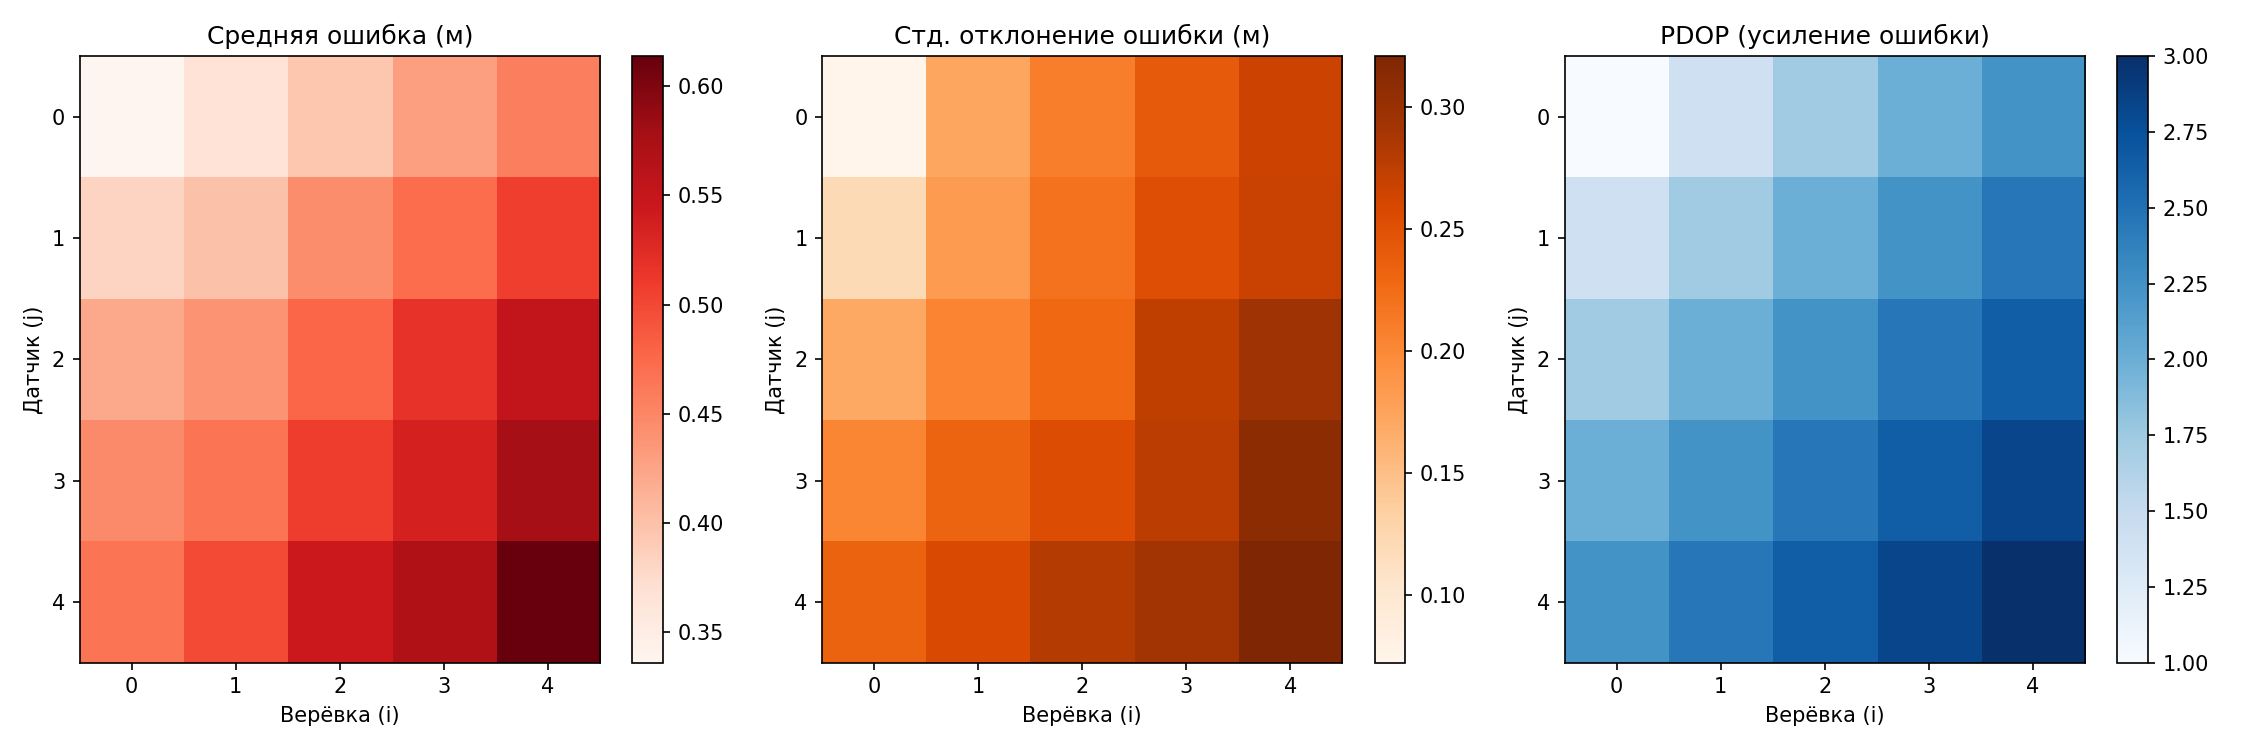
\includegraphics[width=\textwidth]{error_heatmap_detailed.png}
        \end{column}
    \end{columns}
\end{frame}

\end{document}